% Stanford University PhD thesis style -- modifications to the report style
% This is unofficial so you should always double check against the
% Registrar's office rules
% See http://library.stanford.edu/research/bibliography-management/latex-and-bibtex
% 
% Example of use below
% See the suthesis-2e.sty file for documentation
%
\documentclass[12pt]{report}
\usepackage{suthesis-2e}  % (modified) Stanford thesis style file

% useful packages
\usepackage{graphicx}  % figures
\usepackage{gensymb}  % \degree
\usepackage{siunitx}  % SI units
\usepackage{tabularx}  % nice single page tables
\usepackage{longtable}  % tables spanning multiple pages
\usepackage{hyperref}  % URLs
\usepackage[autostyle, english = american]{csquotes}  % quote orientation
\MakeOuterQuote{"}

% use png first, otherwise pdf
% (useful for faster compile times, for final submission switch order)
\DeclareGraphicsExtensions{.png,.pdf}
\begin{document}
\title{Generation and Inheritance of Diversity \newline in the Immune Human System}
\author{Michael Aaron Swift}
\dept{Chemical and Systems Biology}
\principaladviser{Stephen Quake}
\firstreader{Daniel Jarosz}
\secondreader{Daria Mochly-Rosen}
\thirdreader{Bali Pulendran}
% \thirdreader{Jane Supernumerary}  % uncomment if needed
% \fourthreader{Severus Snape}  % uncomment if needed
 
% no signature or copyright pages in online submission
% (they are added by the library)

% including chapters, no .tex extension necessary
\beforepreface
\prefacesection{Abstract}
This PhD thesis delves into the intricate mechanisms governing cell differentiation, lineage determination, and migration dynamics in the human immune system, particularly in B and T cells. The research is primarily based on three major contributions that employ single-cell transcriptome sequencing, lineage tracing, and immune repertoire sequencing techniques.

The first contribution details work I did to create Tabula Sapiens: a comprehensive human reference atlas that encompasses nearly 500,000 cells across 24 different tissues and organs. By analyzing the molecular characteristics of over 400 cell types and their distribution, the atlas enables the identification of tissue-specific gene expression and clonal distribution of T cells. The study also investigates B cell mutation rates and class-switch recombination in various tissues.

The second contribution investigates the role of cell-intrinsic factors in determining cell fates and differentiation outcomes during in vitro B cell activation. By analyzing lineage relationships and single-cell RNA sequencing measurements, the study uncovers the transcriptional programs underlying cell-intrinsic clonal fate biases and the interaction between extrinsic signals, intrinsic state, and clonal population structure. 

The third contribution uses the same techniques to explores the dynamics of B cell migration and clonal expansion in multiple tissues from six donors. The findings reveal the most detailed picture have of the B cell system in humans. We find a tight scaling between lineage size and migration probability, with larger lineages exhibiting a greater likelihood of migration. Moreover, our work sheds light on the sharing of clones and lineages between tissues and the impact of local micro-environmental cues on gene expression in the bone marrow.

By integrating these multi-modal single-cell analyses, this thesis significantly sharpens our understanding of the complex processes governing cell differentiation, lineage determination, and migration in the human immune system. 
\prefacesection{Acknowledgements}
I am deeply grateful to my advisor, Steve Quake, for his unwavering belief in his students and his kind guidance. Steve's contributions to the work presented here have been invaluable, as has been his role in my growth as a scientist. The fun, hard-working, and rewarding environment he has cultivated in his lab is something I greatly appreciate. What I admire most about Steve is his broad range of interests and his incisive lines of questioning.

My sincere thanks go to my committee members, Dan Jarosz, Daria Mochly-Rosen, and Bali Pulendran, for their insightful guidance and probing questions. I would also like to express my heartfelt gratitude to Felix Horns. His contribution to my development as a graduate student cannot be overstated. From him, I have learned about single-cell sequencing, the molecular biology underpinning these technologies, and bioinformatics. He taught me how to think critically about data and read scientific literature carefully. His patience as I navigated my learning journey, and his qualities as a collaborator, mentor, and friend, are deeply appreciated.

I extend my thanks to Bob Jones and Sheela Crasta for their help in coordinating sample collections for the Tabula Bursa work, and to the anonymous organ donors who made this work possible. I am grateful to Norma Neff, Rose Yan, and Angela Detweiler for their assistance in generating most of the sequencing data presented here, and to Ivana Cvijovic for being a fantastic collaborator and friend.

I express my gratitude to all members of the Quake group. Despite the high turnover in academic labs, the soul of our lab — always curious and courageous in the pursuit of science — has remained constant. Working with this team has been a joy. I would like to give special thanks to Mira Moufarrej, with whom I shared a bay. Her company made coming to work enjoyable, and her help with computational and experimental issues was invaluable.

I thank Whitney Combes, Vickie Lin, and Sheela Crasta for their roles in keeping the lab running smoothly. My work was supported by an NIH training grant and a National Science Foundation Graduate Research Fellowship, for which I am grateful. Lastly, but by no means least, I thank my friends and family for their support throughout my graduate school journey. In particular, I want to acknowledge my Mom and Dad, the most supportive people I've ever known. I love them dearly.
\afterpreface
\chapter{Introduction}

\section{Background}

\section{The promise of single-cell biology}
Biology is a watery, messy soup. The cell, mostly a bag of water filled with a generous portion of biological macromolecules like proteins and nucleic acids, is a hub of continuous, seemingly random, riotous motion \cite{berg1993random}. This randomness, while seemingly chaotic at the microscopic level, is statistically reproducible on the cellular and organismal scale, enabling life to reproduce itself. Ensembles of proteins and cells work in organized unison to create functional and successful organisms, such as the one reading this thesis. A key question in biology is how these ensembles work.

We have some reasonable answers to this question. In human biology, for instance, there are around 20,000 genes in the genome. Each cell translates a subset of these genes into proteins, and the identity of these proteins determines a cell's form and function. Broadly, the differential presence and abundance of these proteins and their post-translational modifications are what make a neuron, for instance, different from a blood cell. As far as we know, blood cells do not become neurons, even though they have the genes available. Instead, cell types maintain their identities. During development, these cellular identities are established early and are often maintained throughout the life of the organism. While this model is broadly explanatory, the long-standing goals of biology include understanding which molecules are expressed in cells, when this expression occurs, and how it is maintained.

To return to the bag metaphor: how does this messy bag of water and biomolecules create an organism comprising thousands of distinct bags working in autonomous unison? This question is fascinating in and of itself, but the benefits of developing a deep understanding of development are immediately practical. A real understanding of these molecular processes would allow us to program biology towards the goal of eliminating human diseases. A major target for such reprogramming efforts is the human immune system, which is in a constant state of development and diversification.

Recently, single-cell sequencing technologies have been developed that allow us to define the molecular processes at work in cells by comprehensively measuring which molecules are present. In this thesis, I used these technologies to build a quantitative understanding of the diversity of cell types and proteins in the human immune system. I pursued this goal in three related projects.

The first project aimed to create a comprehensive parts-list for human biology. Specifically, we abstracted the cellular bag as containing just RNA \cite{quake2021cell}: what's in the bags? The second project measured the maintenance of B cell identities and bias during cellular reprogramming: if the contents of the bag must change, how is the identity of the bag maintained? The third project aimed to understand the statistics that describe and govern the dynamics of the human B cell repertoire: what governs the decisions of the bags to change their composition and location in the body?


\section{A Parts-List for Human Biology}
In the first part of my thesis, I collaborated with the Tabula Sapiens consortium to capitalize on recent advances in our ability to systematically measure the identities of macromolecules in single cells. This parts-list approach to biology allows for a systematic understanding of the various functions cells can perform. To use an analogy, if an organism were a kitchen, we are now able to classify all the appliances within by enumerating the parts in each. We now understand what parts make up the toasters, refrigerators, and blenders of biology. Specifically, I employed recent advances in single-cell RNA sequencing techniques to quantify gene expression and cellular identities at the individual cell level \cite{klein_droplet_2015, macosko2015highly}, an ideal level of abstraction for understanding tissue and organismal biology. As I detail in this chapter, we created one of the broadest single-cell references in existence \cite{tabula_sapiens_consortium_tabula_2022}, complemented by other more focused efforts \cite{dominguez_conde_cross-tissue_2022}.

\section{Lineage Tracing during Cell Reprogramming}
In the second part of my thesis, I used B cells as a model to quantitatively understand the maintenance of cell-intrinsic identities as cells differentiate. Phil Hodgkin and his associates have made significant contributions to our understanding of immune cell development and function through the application of lineage tracing techniques \cite{hodgkin2012cell, marchingo2014t}. With the advent of immune repertoire sequencing and single-cell RNA sequencing, researchers can now perform high-resolution clonal lineage tracing, linking cellular differentiation processes to gene expression profiles of lineages of cells \cite{stubbington2017t, horns2020memory}. In this work, I quantify the strong intrinsic fate biases of different types of B cells to the same stimulus, describe the extent to which transcriptional memory is passed through generations of B cells, and characterize the magnitude of this effect in Bone-Marrow Derived Plasma Cells \textit{in vivo}.

\section{Lineage Tracing the B Cell Repertoire across Tissues}
In the third part of my thesis, I collaborated with Ivana Cvijovic on a project to map the statistics of the human B cell repertoire. These statistics prove useful for building models of how B cell differentiation proceeds in humans. This work builds on the work in Chapter 2 by generating a quantitative single-cell genomics dataset for B cell repertoire analysis. We procured immune-rich organs (spleen, lymph nodes, blood, and bone marrow) from otherwise immunologically healthy individuals and processed these cells via single-cell RNA sequencing. Using the lineage information contained in the antibody sequence, we were able to reconstruct lineage histories, and thus the human B cell differentiation process.

\section{Thesis Overview}
The chapters of this thesis focus on research I conducted on similar but distinct topics, as outlined above. Each chapter is arranged to stand as its own document. Much of the work in each chapter is published (Chapters 2 and 3) or will soon be published (Chapters 4 and 5).
% Full title as you would like it to appear on the page
\chapter{Tabula Sapiens: A molecular atlas of human cells}
% Short title that appears in the header of pages within the chapter
\chaptermark{Tabula Sapiens}

\section{Abstract}
Single-cell transcriptome sequencing will help biologists understand the molecular characteristics and physiological functions of human organs. In this study, we constructed the Tabula Sapiens, a comprehensive human reference atlas containing nearly 500,000 cells from 24 distinct tissues and organs. My analysis enabled the molecular characterization of over 250,000 immune cells, their distribution across tissues, and tissue-specific gene expression variations. By examining multiple tissues from a single donor, I investigated the clonal distribution of T cells, tissue-specific mutation rates in B cells, and tissue-specific gene expression programs of multiple cell types. The Tabula Sapiens provides a valuable resource for studying gene expression programs and lineage histories of shared cell types across tissues, opening up new avenues for understanding human physiology and disease. The clone tracing I performed in T cells in this work is an important proof-of-concept for the following chapters, where I use lineage tracing of B cells to gain insight into the dynamics of the human immune system. 

\section{Introduction}

The Tabula Sapiens project represents a significant milestone in the study of human biology(Figure \ref{fig:TabulaSapiens_summary}). By leveraging cutting-edge technologies such as single-cell capture via microfluidics, high throughput DNA/RNA sequencing, and immune repertoire sequencing, this project provides researchers with valuable insights into cellular taxonomy, tissue structure, cell fate and lineage, and cellular communication. Ultimately, the Tabula Sapiens project can revolutionize our understanding of human biology, inform the development of novel therapeutic strategies, and facilitate early detection and diagnosis of various diseases. Importantly, this effort is mainly a reading project. We generated a parts-list for human biology at unprecedented scale and depth. However, a revolution in biology critically depends upon our ability to write biological information and reprogram cells at a similar scale.  

\begin{figure}[hbt!]
\centering
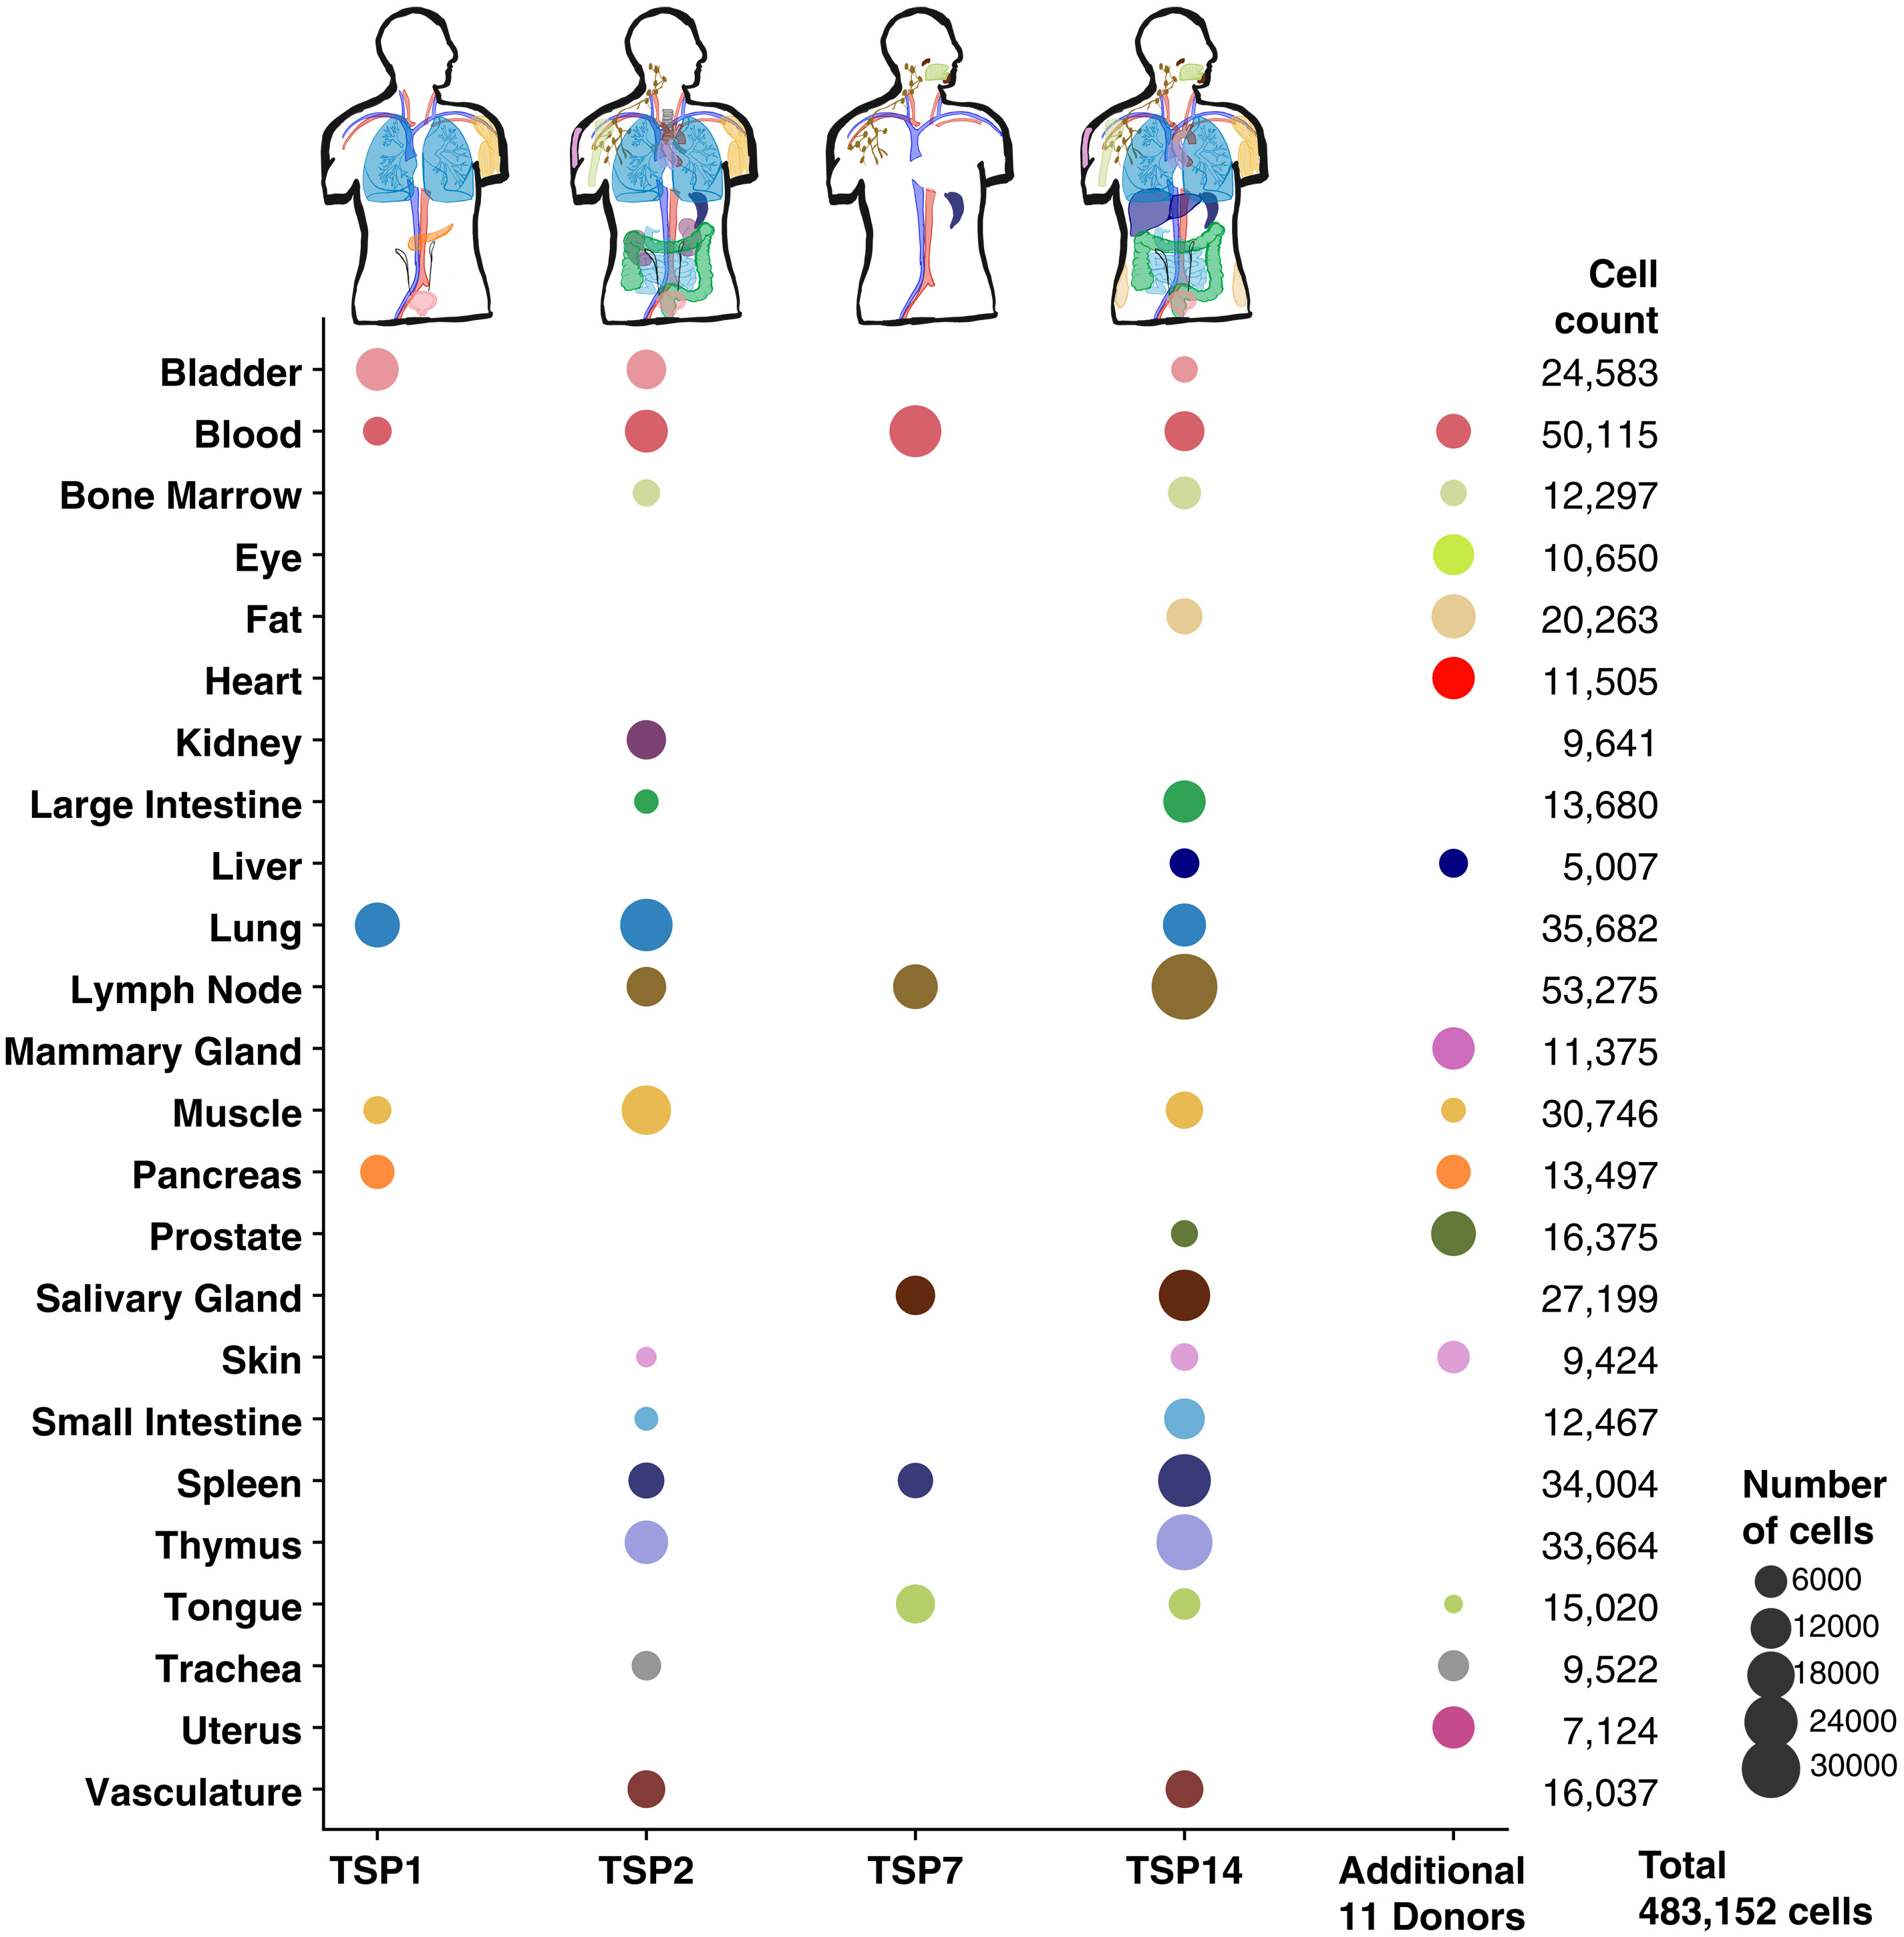
\includegraphics[width=8cm, keepaspectratio]{figs/TabulaSapiens/fig0_Tabula_Summary.jpg}
\caption[ Overview of Tabula Sapiens.]{The Tabula Sapiens was constructed with data from 15 human donors; for detailed information on which tissues were examined for each donor, please refer to table S2. Demographic and clinical information about each donor is listed in the supplementary materials and methods and in table S1. Donors 1, 2, 7, and 14 contributed the largest number of tissues each, and the number of cells from each tissue is indicated by the size of each circle. Tissue contributions from additional donors who contributed single or small numbers of tissues are shown in the additional 11 donors column, and the total number of cells for each organ are shown in the final column on the right.}
\label{fig:TabulaSapiens_summary}
\end{figure}

\subsection{Motivation for the Tabula Sapiens}

Our knowledge of the cells that make up the human body, as well as their variations across individuals, developmental stages, and health or disease states, remains limited. The Human Cell Atlas (HCA) initiative is loosely-affiliated global collaboration involving scientists from numerous universities and institutes. Tabula Sapiens is a part of this broader effort, which aims to address this knowledge gap by creating comprehensive reference maps of all human cells\cite{regev2017human} These maps will serve as a foundation for research, diagnosis, monitoring, and treatment, providing crucial insights into cellular taxonomy, histology, developmental biology, physiology, and even comparative evolution.

Technological advancements have allowed the construction of a systematic molecular atlas at an unprecedented resolution. Single-cell RNA sequencing, for example, now the measurement of  mRNA profiles for millions of individual cells\cite{svensson2017power}. Other techniques, such as those assessing protein molecules\cite{stoeckius2017simultaneous} and chromatin accessibility\cite{buenrostro2015atac}, further contribute to the wealth of information obtained from each cell. These tools have already shown tremendous potential in early studies, leading to the discovery of new cell types in various organs and tissues and providing insights into the immune system and tumor ecosystems\cite{regev2017human}.

\subsection{Tabula Sapiens and the Development of Key Technologies}

The Tabula Sapiens project builds upon the foundation laid by the HCA initiative, taking advantage of recent technological advancements in single-cell capture, sequencing, and immune repertoire sequencing. Microfluidics-based single-cell capture techniques have revolutionized the isolation and analysis of individual cells, allowing for the high-throughput processing and in-depth investigation of cellular heterogeneity\cite{macosko2015highly, klein_droplet_2015}. DNA/RNA sequencing technologies have similarly evolved, enabling the rapid and cost-effective characterization of an organism's entire genome or transcriptome\cite{goodwin2016coming}. Immune repertoire sequencing has also seen significant progress, facilitating the in-depth exploration of adaptive immune responses by analyzing the diversity of B and T cell receptors\cite{georgiou_promise_2014}.

Together, these technologies have empowered researchers to embark on the Tabula Sapiens project, an endeavor that will greatly enhance our understanding of human biology and provide a foundation for future research, diagnosis, and treatment. The integration of these technologies will help address key challenges in diverse biological fields, as well as facilitate the development of better drugs and more accurate predictions of unintended toxicity. Ultimately, the Tabula Sapiens project will contribute to a more comprehensive understanding of human cells and their functions, driving innovation in regenerative medicine and diagnostic tests.

\subsection{My contributions to the project}
In this study, I made a significant contribution to the Tabula Sapiens project, a comprehensive effort to generate a human cell atlas covering all major tissues and cell types. My involvement in the project spanned from collecting tissues, to analyzing data,  and writing the manuscript. included three primary aspects: collecting tissues and creating single-cell suspensions including developing a protocol to isolate bone marrow cells from human vertebral bodies, generating and advising in the preparation of 10X Genomics libraries, and performing tissue-specific gene expression analysis and clonal analysis of T cells, as well as estimating important parameters of B cell population genetics across tissues.

First, I successfully developed a novel protocol to isolate bone marrow cells from human vertebral bodies, a challenging tissue source due to the intricate structure and limited accessibility of the vertebral bone marrow. This protocol enabled me to obtain a high-quality, representative cell population from this complex tissue, thereby enriching the Tabula Sapiens project with essential data on bone marrow cell types and their interactions. Additionally, I processed lymph nodes, spleens, and blood for various Tabula Sapiens donors.

Second, I played a crucial role in generating and troubleshooting 10X Genomics and Smart-seq2 libraries for the project. My expertise in scRNA-seq library preparation allowed me to generate the 10X 5prime data efficiently and well as serve in a key advisory role for the rest of library preparation optimize conditions and workflow, ensuring the generation of high-quality, reproducible data.

Finally, I performed tissue-specific gene expression analysis and clonal analysis of T cells, as well as estimated important parameters of B cell population genetics across tissues. My tissue-specific analysis helped uncover unique gene expression patterns and functional states of T and B cells in different human tissues. I investigated the clonal relationships among T cells and provided a view into their tissue-specific expansion and functional roles. Additionally, I estimated key parameters of B cell population genetics, such as somatic hypermutation rates and class-switch recombination frequencies, across various tissues, providing a view of B cell dynamics in human health and disease. 


\section{Results}

\subsection{Tissue-Specific Gene Expression Signatures of Immune Cells}

We performed a differential gene expression analysis on the immune cell types across all of the tissues, revealing tissue-specific gene expression signatures of immune cells. Although we identified signatures of interest for most cell types in our dataset, here we focus here on the 36,475 macrophages distributed amongst 20 tissues. Using PCA on the top 300 differentially expressed genes in macrophage across all tissues, we show a number of highly distinct macrophage subtypes (Figure \ref{fig:TabulaSapiens_gex}A). PCA distinguished lung and lymph node macrophages from all other macrophages, driven largely by the high expression of CHIT1 and anti-microbial genes. Macrophage in the spleen were unique amongst tissues, expressing SPIC and CD5L. This suggests that most macrophages in the spleen are red-pulp macrophages. Additionally, we identified a gradient of EREG expression that distinguished tissues such as skin, uterus, and mammary tissues from circulating macrophages in the blood (Figure \ref{fig:TabulaSapiens_gex}B). EREG, secreted by macrophages, is thought to participate in cancer progression and facilitate the tumor micro-environment but also has important roles in homeostatic maintenance of tissues. We summarize our analysis by plotting a clustermap of gene expression signatures of the macrophages and their tissue-defining genes (Figure \ref{fig:TabulaSapiens_gex}C), and by providing the gene loadings of the first 4 principal components in our analysis (Figure \ref{fig:TabulaSapiens_gex}D). 
\begin{figure}[hbt!]
\centering
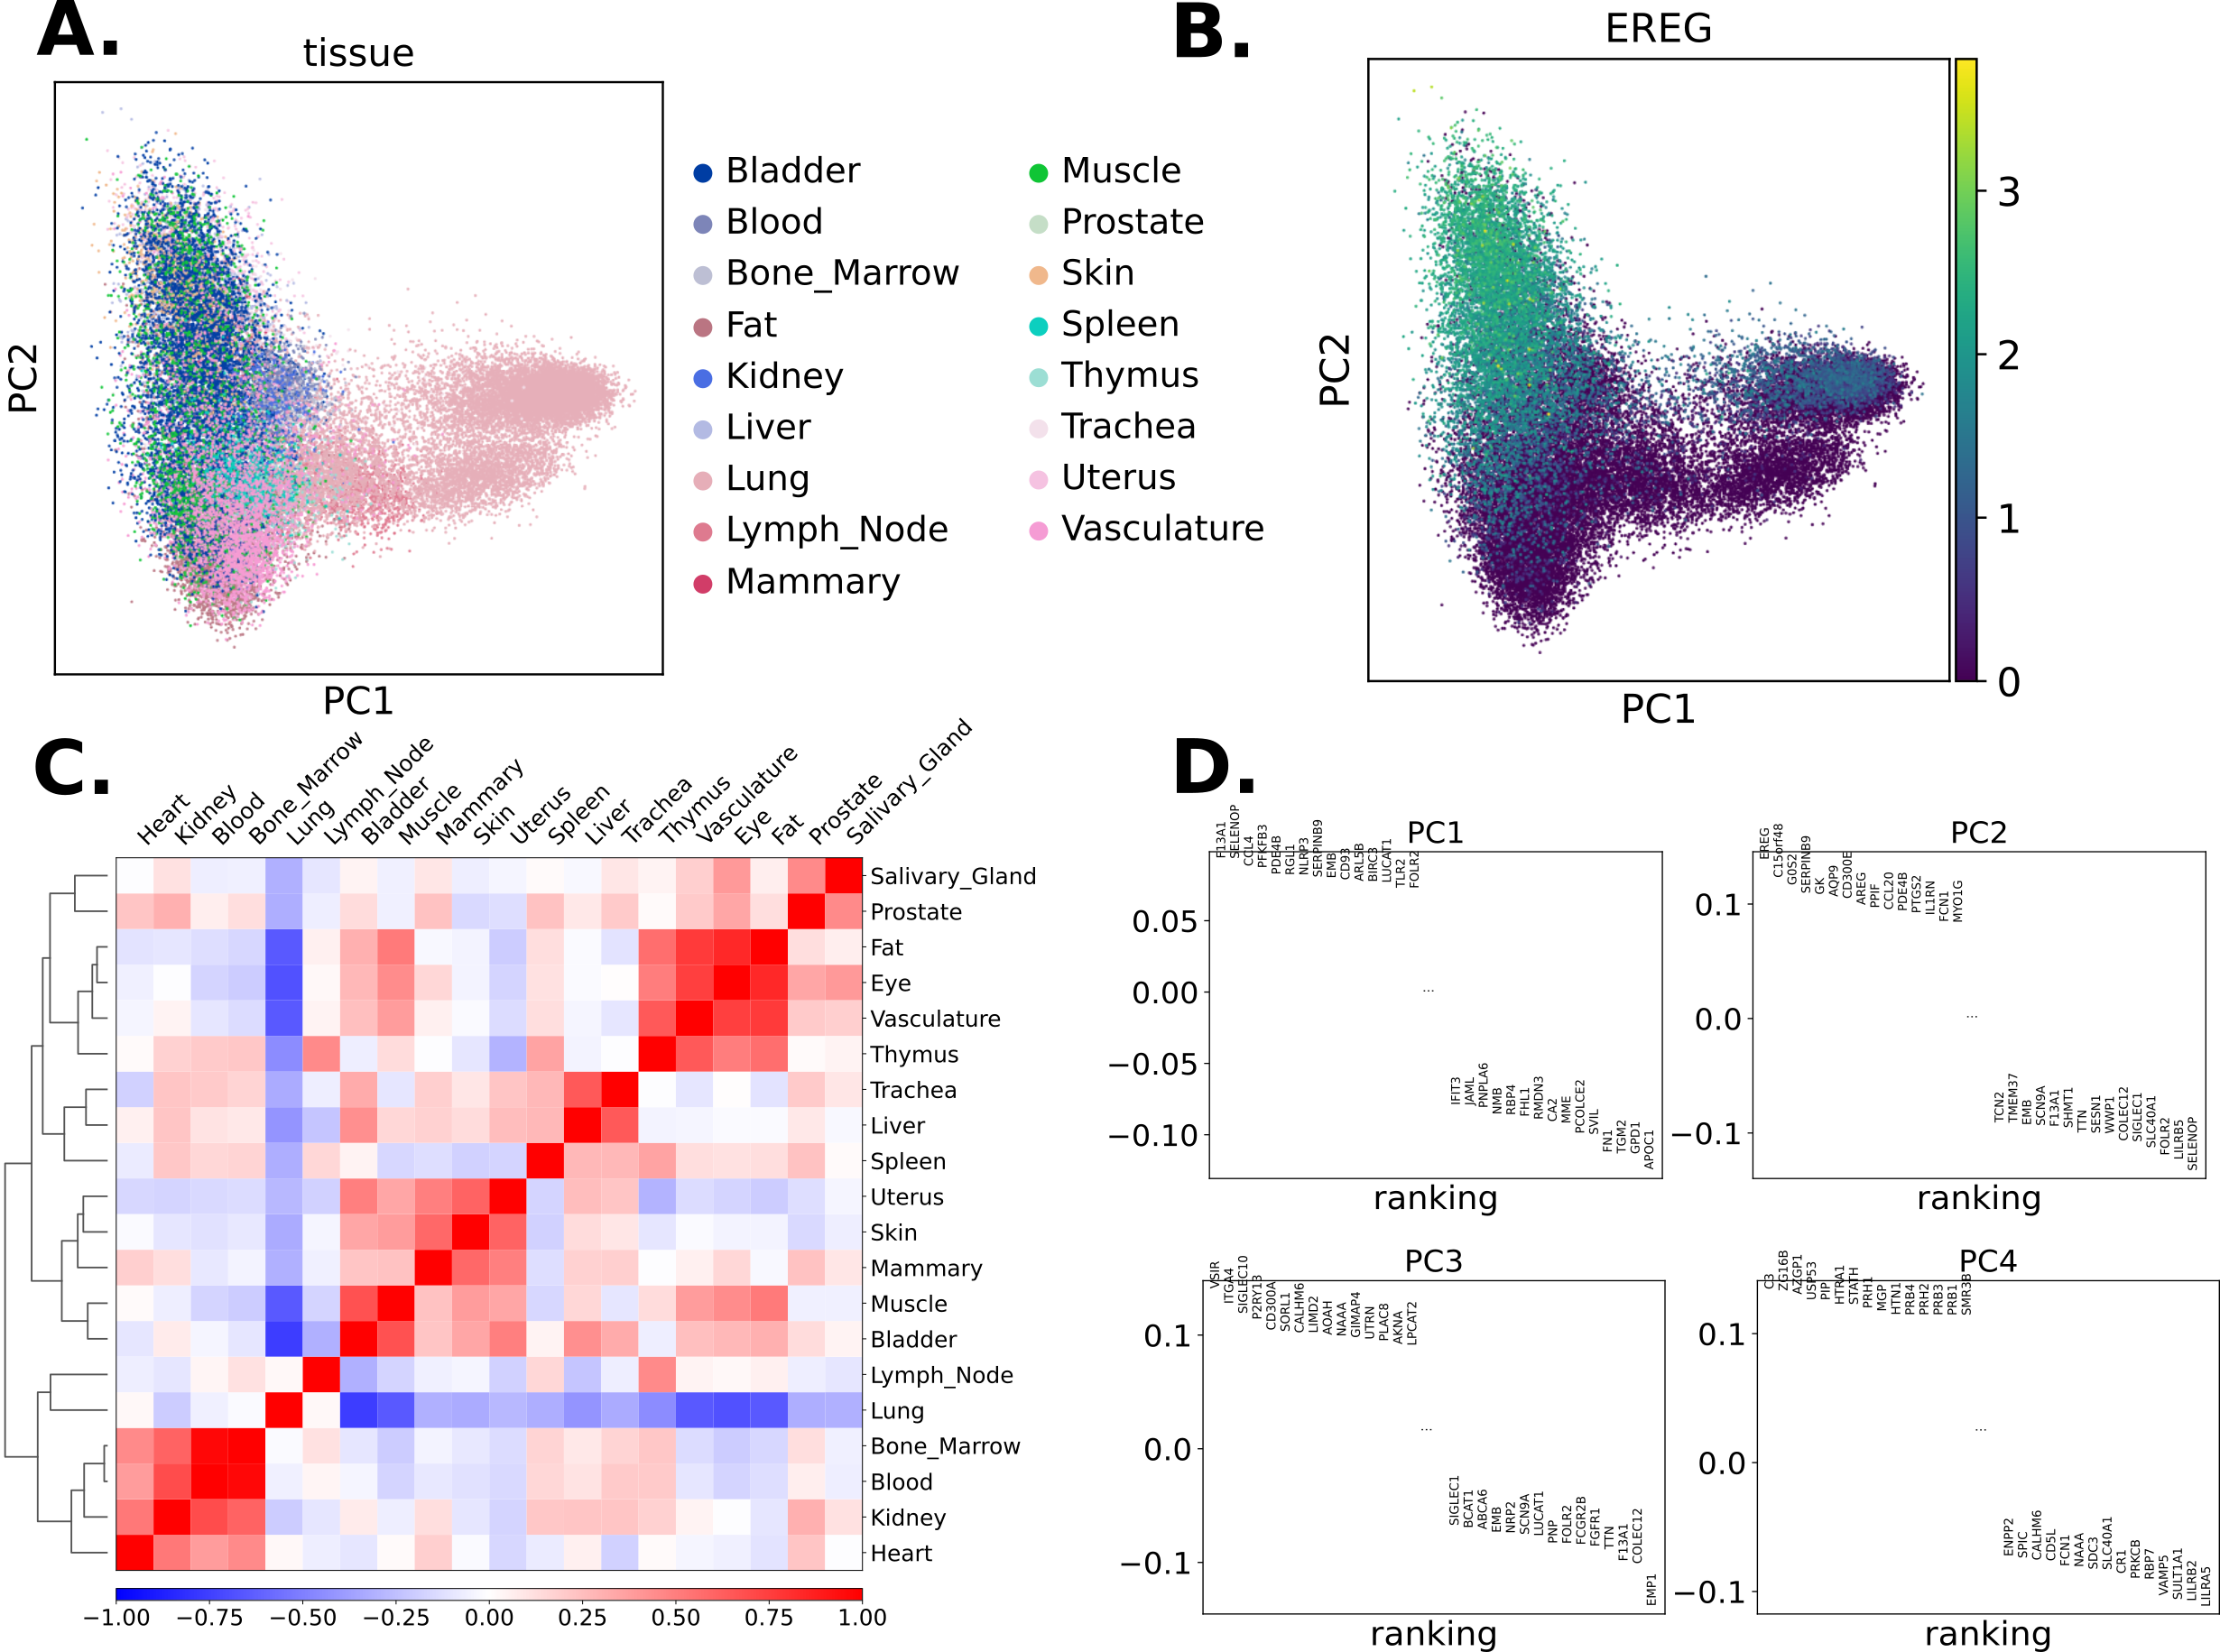
\includegraphics[width=14cm, keepaspectratio]{figs/TabulaSapiens/fig1_gex_analysis.png}
\caption[Gene Expression Analysis of Tissue Resident Macrophage]{(A) PCA projection of the top 300 differentially expressed genes amongst macrophage amongst tissues. (B) Epiregulin expression defines macrophage residence in stromal tissues. (C) Correlation matrix of tissue resident macrophage gene expression. (D) Gene loadings of the first 4 principal components of gene expression variation amongst macrophage}
\label{fig:TabulaSapiens_gex}
\end{figure}

\subsection{Background the Adaptive Immune System}
Our analysis aimed to elucidate the molecular details of immune cell trafficking within individual humans by comparing different immune cell subsets across various tissues. These cells are known to originate in specific niches, circulate throughout the body, and home to other niches where they can remain for on time-scales ranging from minutes\cite{jerison_heterogeneous_2020} to years\cite{hammarlund_plasma_2017}. The adaptive immune system consists of T cells and B cells which mount a specific response to pathogens and vaccines. B cells produce antibodies and T cells direct attack infected cells through the MHC system. These lymphocytes express relatively unique receptors on their cell surface (BCRs and TCRs)(Figure \ref{fig:TabulaSapiens_airr}A), which are created in a stochastic process which results in the creation of diverse gene combinations\cite{alberts2017molecular}. Thus, lymphocytes are relatively uniquely marked at the time of their origin, such that observation of the same sequence in two cells indicates a clonal relationship between them. In order to identify these clones by their immune receptor, we needed to sequence the TCR or BCR. The techniques for sequencing TCRs and BCRs are called Airr-seq, or Adaptive Immune Receptor Repertoire sequencing. It is a high-throughput sequencing method that enables the in-depth analysis of the T cell receptor (TCR) and B cell receptor (BCR) repertoires of the adaptive immune system. 

\begin{figure}[hbt!]
\centering
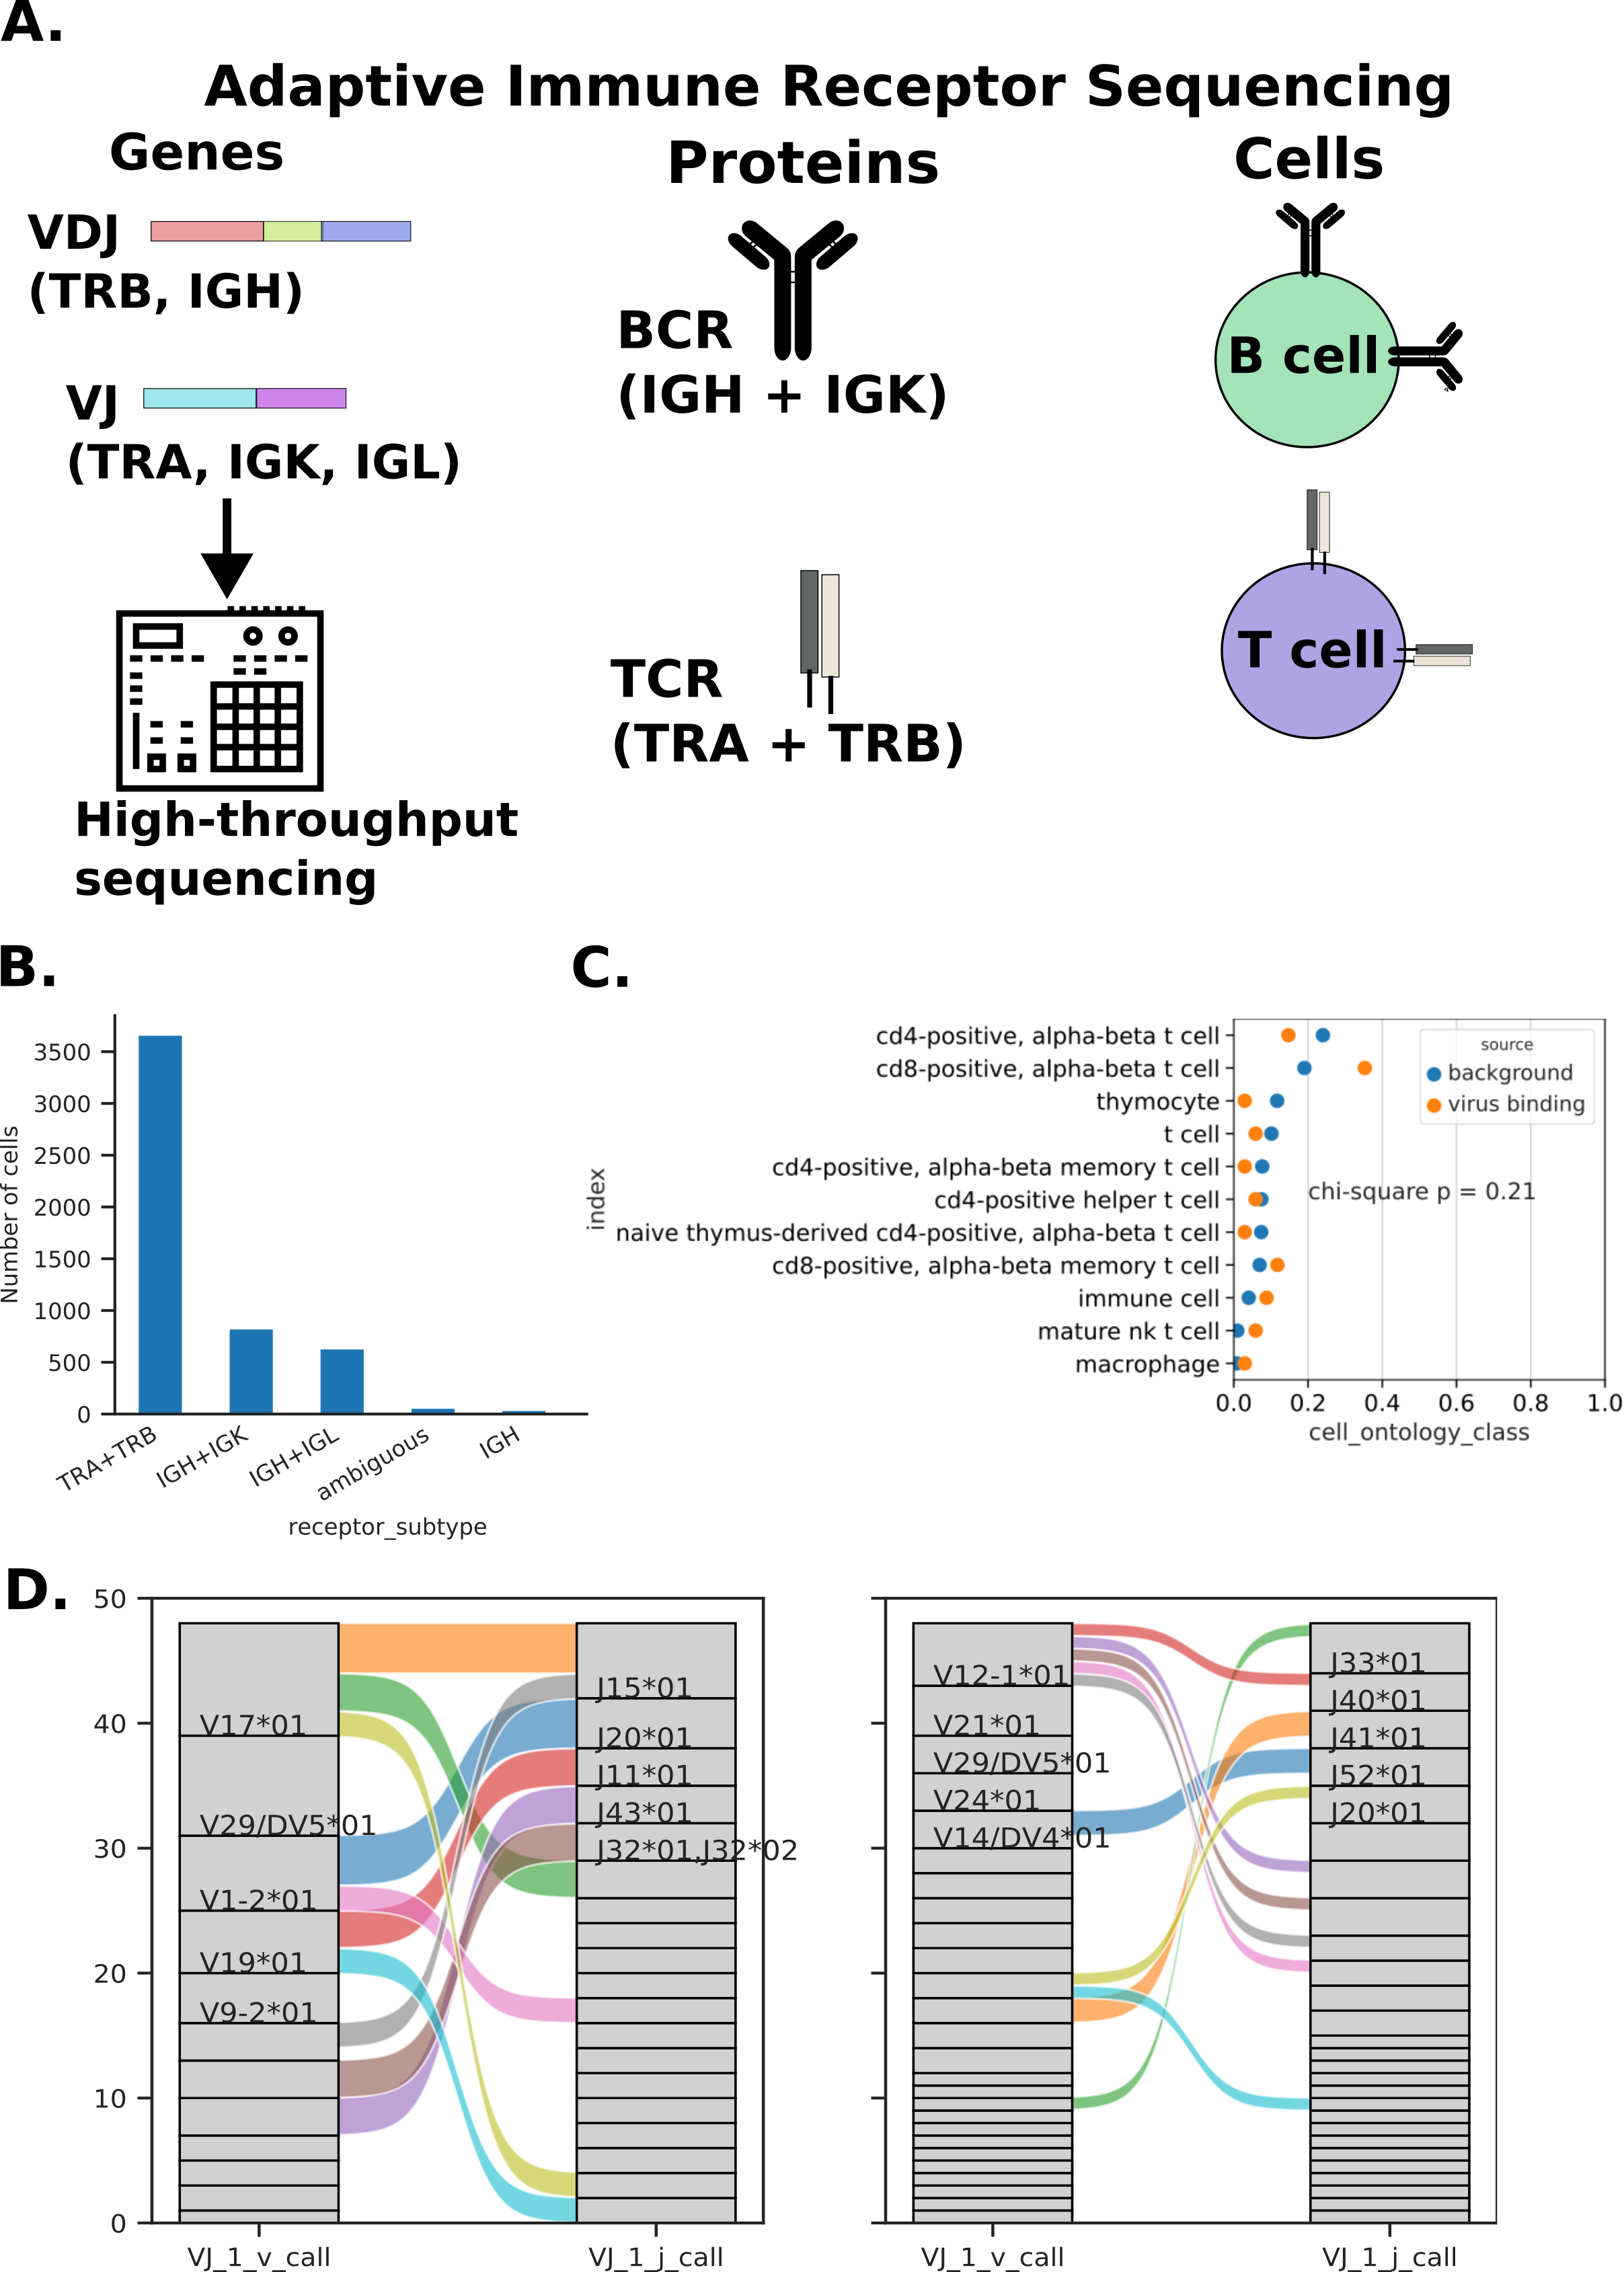
\includegraphics[width=10cm, keepaspectratio]{figs/TabulaSapiens/fig2_tabula_airr.png}
\caption[AIRR-seq for analyzing the T cell Repertoire in Tabula Sapiens]{A. Schematic of AIRR-seq. B. Countplot of TCRs and BCRs computationally assembled from Smart-Seq2 and 10X 5prime data. MAIT cells and other invariant T cells use a stereotypical repertoire of V and J genes. Multi-donor T cell clones (left) tended to use a restricted set of known MAIT genes as compared to the (downsampled for comparison) full T cell repertoire (left)}
\label{fig:TabulaSapiens_airr}
\end{figure}



\subsection{Computational Analysis of TCR and BCR from single cells}
We attempted computational assembly of TCR and BCR for all cells sequenced via Smartseq2 and the subset of cells sequenced using the 10X 5' system. Our pipeline yielded order thousands of TCRs and BCRs for analysis (Figure\ref{fig:TabulaSapiens_airr}B). We also investigated where convergent T cell clones could be detected amongst donors. Since VDJ recombination proceeds stochastically and relatively uniquely in each donor, similar VDJ recombination signatures across donors would suggest there are certain cases where a limited repertoire of recombination genes is used. Using the VDJ recombination signature of T cells, we found that multi-donor T cell clones did indeed tend to use a restricted set of genes known to be used by Mucosal Associated Invariant T cells(Figure\ref{fig:TabulaSapiens_airr}D). 

\subsection{Cross-Referencing TCR/Epitope Pairings with Tabula Sapiens}

We downloaded a curated database of TCR/epitope pairings containing 54,181 unique CDR3-to-epitope pairings from \url{https://vdjdb.cdr3.net/}. The majority of these pairings are supported by evidence from dextramer, tetramer, or multimer sorting and subsequent sequencing. In some cases, this data is derived from single-cell analysis, while in others, it is based on bulk RNA. We then cross-referenced this database with the Tabula Sapiens database of TCRs that we generated. Upon cross-referencing, we identified 25 TCR Beta Chains with exact matches in the database describing TCR/epitope pairings (Table \ref{tab:TabulaSapiens_tab1_viral_peptides}). This represents roughly 1/100 of the TCRBs in Tabula Sapiens. We exclusively identified TCRs that are likely to bind viral peptides, as opposed to self-peptides.

\renewcommand{\arraystretch}{2}  % make spacing nicer
\begin{table}[hbt!]
\centering
\begin{tabularx}{10cm}{cc}  % 2 columns center-justified
   \textbf{Virus} & \textbf{Number of Peptides} \\
   \hline  % horizontal line
Epstein-Barr Virus (EBV) & 12 peptides \\
\hline
 Cytomegalovirus (CMV) & 8 peptides \\
\hline
Influenza A & 5 peptides \\
\hline
\end{tabularx}
\caption[Table of TCR-Binding Inferences]{We cross-referenced the TCRs identified in Tabula Sapiens with the VDJdb to infer whether any TCRs we identified may bind viral peptides}
\label{tab:TabulaSapiens_tab1_viral_peptides}
\end{table}

\subsection{Distributions of Virus-Binding T Cells}
The EBV-binding T cells were found in donors TSP2 and TSP7. In TSP7, the single EBV-specific T cell was located in the tongue. In TSP2, EBV-specific T cells were distributed amongst multiple immune organs. We could not perform any meaningful statistical comparison with such low numbers of cells. We also analyzed the cell types for virus specific T cells. We found a subtle enrichment of CD4 and CD8 T cells associated with viral peptide binding TCRs (Figure\ref{fig:TabulaSapiens_airr}C). This enrichment was not significant, but likely would be given more cells to analyze.

Finally, we visualized the distribution of T cell clones across the tissues we sampled for TSP2, the donor which had the most T cells available for analysis. We represented these tissue-clone relationships with a Sankey plot, that shows the networks of T cell clones shared by different tissues in the body(Figure\ref{fig:TabulaSapiens_sankey}). In particular, there appears to be network of clones which move between the Bone Marrow, Spleen, and Blood. Additionally, when clones are large enough, they are readily detectable in many disparate tissues (e.g. clone m, Muscle and Spleen), suggesting broad movement of large clones throughout the body    
\begin{figure}[hbt!]
\centering
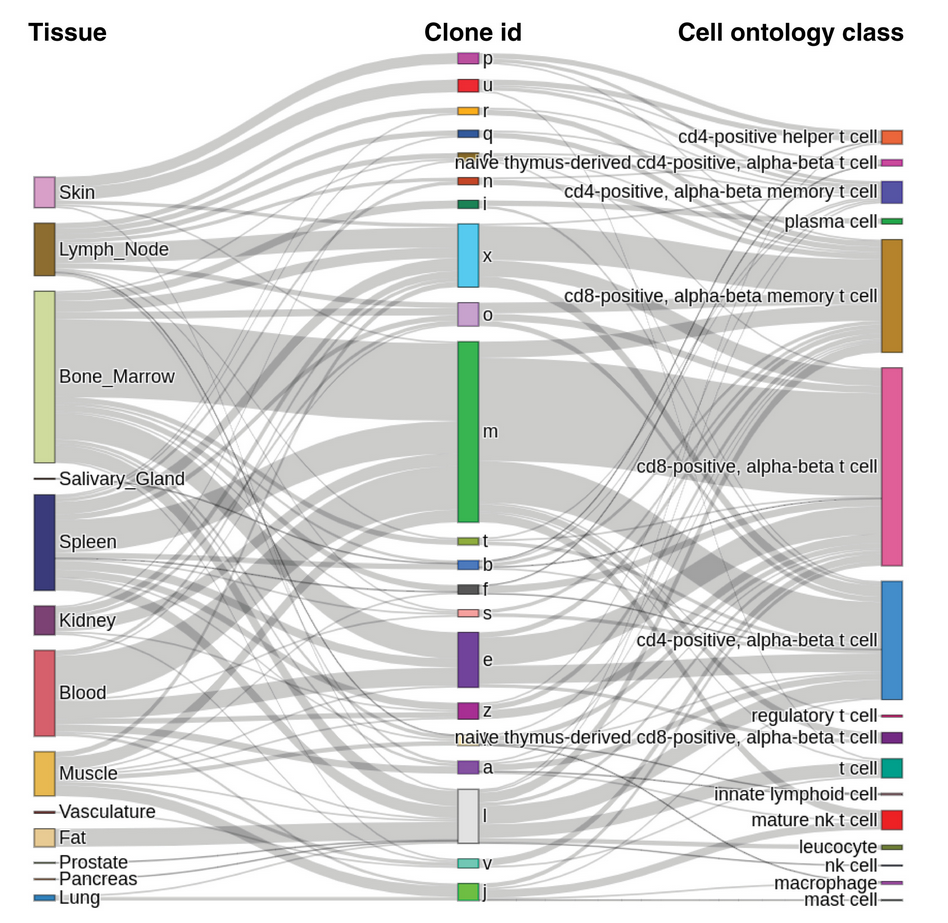
\includegraphics[width=14cm, keepaspectratio]{figs/TabulaSapiens/fig4_sankey.png}
\caption[Sankey Plot of T cell clones in Tabula Sapiens]{Illustration of clonal distribution of T cells across multiple tissues. The majority of T cell clones are found in multiple tissues and represent a variety of T cell subtypes. nk cell, natural killer cell.}
\label{fig:TabulaSapiens_sankey}
\end{figure}



\subsection{Isotype Distribution in B Cells Across Tissues}

B cells secrete different isotypes of the IgH gene, which have different roles in immunity. IgA interacts with pathogens and commensals at mucosal surfaces, IgG is often involved in direct neutralization of pathogens, and IgM is typically expressed in naive B cells or secreted in the first response to pathogens. We classified every B cell in the dataset as expressing IgA, IgG, or IgM and calculated the relative amounts of each isotype in each tissue. This analysis revealed a gradient of IgA expression across tissues, with blood having the least relative abundance of IgA cells and the large intestine having the highest relative abundance (Figure \ref{fig:TabulaSapiens_igh}A).

\subsection{Tissue-Specific Somatic Hypermutation in B Cells}

We measured the level of tissue-specific somatic hypermutation in B cells by computationally assembling the B Cell Receptor (BCR) and then inferring the germline ancestor of each cell\cite{lindeman2018bracer,gupta2015change}. In the bone marrow, we observed a bimodal distribution of hypermutation, consistent with the coexistence of plasma cells and recently birthed B cells (Figure \ref{fig:TabulaSapiens_igh}B). Solid tissues have an order of magnitude higher level of mutations per nucleotide (0.07 ±0.04) compared to the blood (0.007±0.02), suggesting that immune infiltrates of solid tissues are dominated by antigen experienced B cells.

\begin{figure}[hbt!]
\centering
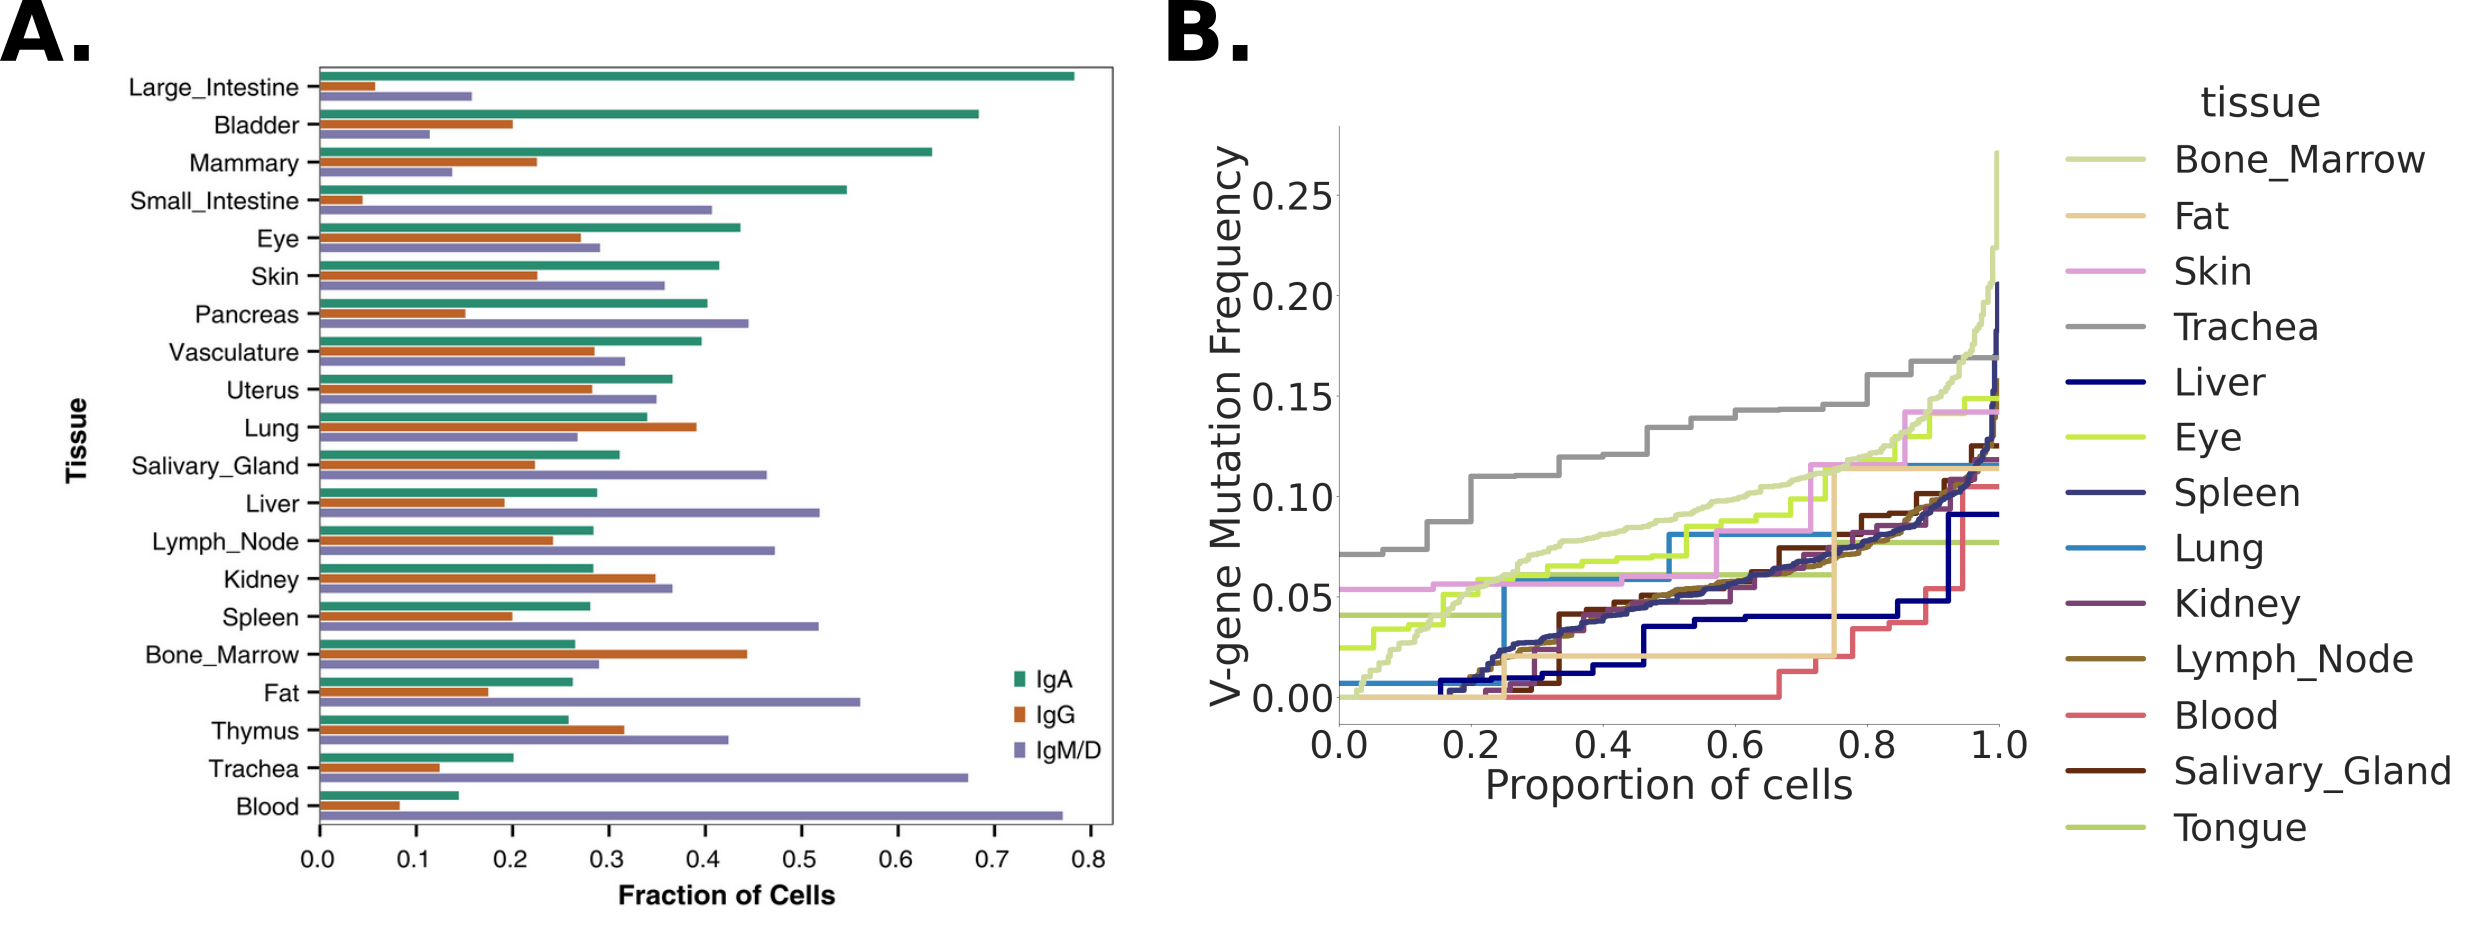
\includegraphics[width=14cm, keepaspectratio]{figs/TabulaSapiens/fig3_tabula_igh.png}
\caption[Tissue population-level parameters of B cell Dynamics.]{(A) Prevalence of B cell isotypes across tissues, ordered by decreasing abundance of IgA (B) Somatic hypermutation frequencies in the V-genes of B cells sampled from different tissues in
Tabula Sapiens.}
\label{fig:TabulaSapiens_igh}
\end{figure}

\section{Conclusions}

Our results provide valuable insights into immune cell trafficking, tissue-specific gene expression signatures, and the distribution of virus-binding T cells across different tissues. We observed tissue-specific gene expression signatures in all immune cells. Here we presented the macrophages, and identified gradients of EREG expression that distinguished tissue-resident macrophages from circulating ones. We used TCR data to analyze the distribution of virus-binding clones in the body, although we were quite limited by low sampling. In the future, higher-throughput efforts profiling T cells across the body should shed light on how tissue resident T cell memory is maintained and distributed throughout tissues. In the case of B cells and the antibody repertoire, we described the tissue-specific differences in B cell somatic hypermutation and isotype distribution. These data prove conceptually, that a much more deeply sampled study of the adaptive immune system at single cell resolution, could provide a detailed description of the differentiation dynamics throughout the tissues in the human body.

\section{Materials and Methods}
\subsection{Vertebral Body Tissue Processing}
The vertebral bodies (VB) were wrapped in a cloth and shipped to Stanford University on ice.
Upon arrival, the VBs were first cleaned using chisels, to remove any attached connective tissue
and fat. To rinse off any remaining cells attached to the exterior of the VB, the VBs were then
transferred to a plastic nalgene containing 50 mL RPMI + 10\% FBS and tumbled in a bone marrow
tumbler for 20 minutes at room temperature. The rinsing medium was discarded and the VBs
were removed from the tumbler, transferred to a large sterile plastic Petri dish, and cut into ½ inch
by ½ inch pieces using bone cutting forceps. The bone marrow pieces were transferred into a
plastic nalgene, to which 100mL of RPMI + 10\% FBS was added. The nalgene was returned to
the bone marrow tumbler and tumbled for 30 minutes at room temperature. The solution
containing the VB was then passed through a 100 $\mu$M strainer into 50 mL falcon tubes. Multiple
strainers were used in case of clogs. After straining, the cells were centrifuged and pelleted at
330g 4°C for 5 minutes. Cells were resuspended in 1x Erythrocyte Lysis buffer, kept 5 minutes
on ice and mixed. Cells were then re-centrifuged for 5 minutes at 330g at 4°C without brakes, in
order to remove plasma and lysed red blood cells. Cells were then ready to count. 10 million bone
marrow cells were stained using an immune lineagePE cocktail containing CD3-PE, CD4-PE,
CD56-PE, CD11b-PE, and CD14-PE, and subsequent MACS with anti-PE microbeads was
performed. One tube of immune lineage positive and one tube of lineage negative cell were
prepared for the 10x. For Smartseq2, cells were stained with anti-CD38-APC, anti-CD34-FITC,
and sytox blue for 30 minutes at 4°C and washed twice with PBS + 10\% FBS. A more detailed protocol may be found on protocols.io. 
\subsection{BCR and TCR analysis}
\subsubsection{T-Cell processing}
TraCeR\cite{stubbington_t_2016} version 0.5 \url{(https://github.com/czbiohub/nf-tracer)} was used to identify T-Cell clonal
populations. Tracer assemble was run with --species Hsap set. We then ran tracer summarise
with --species Hsap to create the final results. The following versions for TraCeR dependencies
were used: bowtie2 version 2.3.0, igblast version 1.7.0, kallisto version v0.43.1, Salmon version
0.14.1, Trinity version v2.4.0, GRCh38 reference genome. Step-by-step instructions to reproduce
the processing of the data are available from GitHub.
\subsubsection{B-Cell processing}
BraCeR\cite{lindeman2018bracer} version 0.1 \url{https://github.com/czbiohub/nf-bracer)} was used to identify B-Cell clonal
populations. Bracer assemble was run with --species Hsap set. We then ran bracer summarise
with --species Hsap to create the final results. The following versions for BraCeR dependencies
were used: bowtie2 version 2.3.4.1, igblast version 1.4.0, blast 2.6.0, kallisto version v0.43.1,
Salmon version 0.8.2, Trinity version v2.8.5, GRCh38 reference genome. Step-by-step
instructions to reproduce the processing of the data are available from GitHub.
\subsubsection{Data Merging and Immune Repertoire Analysis}
BCR and TCR processing and merging were done via snakemake\cite{koster2012snakemake} and code is available on
github at \url{https://github.com/czbiohub/tabula-sapiens}. Analysis on the snakemake outputs were
performed in JupyterLab. Briefly, all assemblies from cell ranger 6.0.1, tracer, and bracer were
annotated with IgBLAST 1.8.2\cite{ye_igblast_2013} and output in AIRR format. The resulting file was preprocessed
Scirpy\cite{sturm_scirpy_2020} and merged with single-cell gene expression data. Only cells which had a matching
assembly and gene expression data were used for downstream analysis. Scirpy was used to
assign clonotypes with ir.pp.ir\_dist(adata, metric = "alignment”, sequence ="aa”, cutoff = 25) and
ir.tl.define\_clonotypes(adata, key\_added=``clone\_id”). Graphs of clones were created using graph
tool Graph-tool\cite{peixoto_graph-tool_2014}. In the case of 3 prime 10X genomics data, isotypes
were assigned to each B cell by determining the highest expressed immunoglobulin class. Due to a large amount of multi-mapping between sub-isotypes, we
summed the gene expression values in each cell for genes in each class-group (IgA, IgG, IgM/D).
Subtypes were generally not resolvable due to high homology between e.g., IgA1 and IgA2. Otherwise, isotypes labels were taken from the Bracer or Cellranger pipelines.
Somatic Hypermutation Frequencies were calculated as the Levenshtein edit distance from the V-gene sequence
to germline V-call.
\subsubsection{Tissue Immune Signature Analysis}
Genes which were differentially expressed between macrophages residing in different tissues
were identified using sc.tl.rank\_genes\_groups(adata, groupby = ``tissue”, method = ``wilcoxon”).
Genes whose expression is known to be affected by tissue dissociation were removed, see table S9 in the Tabula Sapiens manuscript\cite{tabula_sapiens_consortium_tabula_2022}. Genes were then filtered using sc.tl.filter\_rank\_genes\_groups(adata, min\_fold\_change = 0.8, min\_in\_group\_fraction = 0.5). Genes identified in this manner were then
used as the matrix for subsequent analysis, such as the correlation analysis, cluster-maps, and
PCA. For plotting, the 500 most variable genes identified in the differential tissue expression
analysis, sc.tl.highly\_variable\_genes(adata, n\_top\_genes = 500).
% Full title as you would like it to appear on the page
\chapter{Lineage tracing reveals fate bias and transcriptional memory in human B cells}
% Short title that appears in the header of pages within the chapter
\chaptermark{Lineage Tracing \textit{in vitro}}

\section{Abstract}
We combined single-cell transcriptomics and lineage tracing to understand fate choice in human B cells. Using the antibody sequences of B cells, we tracked clones during \textit{in vitro} differentiation. Clonal analysis revealed a subset of IgM+ B cells which were more proliferative than other B cell types. Whereas the population of B cells adopted diverse states during differentiation, clones had a restricted set of fates available to them; there were two times more single-fate clones than expected given population-level cell-type diversity. This implicated a molecular memory of initial cell states that was propagated through differentiation. We then identified the genes which had strongest coherence within clones. These genes significantly overlapped known B cell fate determination programs, suggesting the genes which determine cell identity are most robustly controlled on a clonal level. Persistent clonal identities were also observed in human plasma cells from bone marrow, indicating that these transcriptional programs maintain long-term cell identities \textit{in vivo}. Thus, we show how cell-intrinsic fate bias influences differentiation outcomes \textit{in vitro} and \textit{in vivo}. 

\section{Introduction}
A key focus of developmental biology is the relationship between the molecular milieu of a progenitor cell and its differentiation outcomes. These outcomes are variously referred to as cell fate, cell identity, or cell state. Lineage tracing offers a powerful way to map which progenitor cells adopt which cell fates. Even rudimentary cell labeling techniques show clonally related offspring are biased toward similar cell fates\cite{whitman_embryology_1878}, and recent technological advances confirm the same with greater throughput and resolution. However, the contribution of cell-extrinsic versus cell-intrinsic molecular factors as determinants of cell fates remains largely uncharacterized.

To better understand cell fate determination, multiple groups have used high-throughput sequencing to measure endogenous or transgenic DNA barcodes as labels of cellular lineage\cite{lu_tracking_2011, naik_diverse_2013}. Recently, it is possible to use high-throughput sequencing to perform both lineage tracing and transcriptomics in single cells. This combination directly measures the molecular relationships between progenitors and their offspring, allowing stronger inference of molecular determinants of cell fates\cite{biddy_single-cell_2018, ludwig_lineage_2019, weinreb_lineage_2020}. For example, by analyzing the transcriptomes of lineages biased towards efficient reprogramming outcomes, Biddy et al were able to identify a previously uncharacterized methyltransferase which increased stem-cell reprogramming efficiency by threefold.

In the human immune system, clonal lineages of leukocytes rapidly proliferate while adopting diverse cell fates. This dynamic occurs \textit{in vivo} as a response to varied pathogenic challenges such as viruses, bacteria, or cancer. Spatially organized cellular structures, called germinal centers, orchestrate this process \textit{in vivo}. However, \textit{in vitro} differentiation protocols using only T or B cells can recapitulate important features of the germinal center, and provide valuable insight into the process\cite{deenick_switching_1999}. \textit{in vitro}, a researcher can control most extrinsic factors, such as cell density, cytokine cocktails, and media compositions, allowing them to study cell-intrinsic differentiation programs. In the case of B and T cells, well-controlled extrinsic conditions still reliably generate a large diversity of cell fates, indicating a strong contribution of intrinsic cell diversity to population-level diversity seen \textit{in vivo}\cite{cheon_cyton2_2021}. The question of how gene expression responds to extracellular stimuli, while a cell maintains its identity, is generally poorly understood. And the transcriptional programs underlying cell-intrinsic clonal fate bias remain largely uncharacterized. Furthermore, how extrinsic signals, intrinsic state, and clonal population structure interact to determine the dynamics of the B cell immune response remains poorly understood.

Here, we gain insight into some of these gaps in knowledge by obtaining lineage and single-cell RNA-sequencing measurements of differentiating human B cells. We used the B cell receptor (BCR) gene as a genetic lineage marker and we paired this information with a transcriptomic readout of cellular identity during an \textit{in vitro} differentiation of human B cells. These multi-modal data allow us to quantitatively infer the intrinsic biases B cells have towards specific cell fates, analyze the clonal dynamics of \textit{in vitro} B cell activation, and characterize transcriptional memory both \textit{in vitro} and \textit{in vivo}.

\section{Pilot Experiments}

To determine the feasibility and utility of lineage tracing and single-cell RNA sequencing, we used Smart-Seq2 to analyze the differentiation and fate choice of human B cells, we stimulated primary naïve B cells with cytokines \textit{in vitro} and performed single-cell RNA-sequencing  (Figure \ref{fig:paper2_prelimfig_1}A). We purified naïve B cells from peripheral blood mononuclear cells (PBMCs) via negative selection against other hematopoetic markers by magnetic cell sorting. Purified cells were 96 \% CD19+ and 97 \% IgD+. We dyed the cells with a division tracking dye called CellTrace Yellow which allowed us to assess their proliferation. The cytokine combination that we used for stimulation, CD40L, IL-2, IL4, and IL21, was shown to induce proliferation, class switch recombination, and differentiation into memory B cells or antibody-secreting cells\cite{konforte_il-21_2009}. After 3, 7, 10, and 14 days, we sorted individual cells into well-plates and performed full-length single cell RNA-sequencing. As a baseline for comparison, we also sorted and sequenced individual purified naive B cells. After quality filtering, we obtained the transcriptomes of 986 stimulated B cells and 364 naive B cells for further analysis.

\subsubsection{Differentiating Naive B cells have diverse transcriptional states}

Dimensionality reduction by principal components analysis (PCA) and UMAP\cite{mcinnes_umap_2018} of single cell transcriptomes revealed several transcriptionally distinct states, which we annotated based on known and novel markers  (Figure \ref{fig:paper2_prelimfig_1}B). Unstimulated cells were distinguished by their high expression of known naïve B cell markers such as IGHD and TSC22D3. The Early-Activation cluster was characterized by expression of secreted cytokines such as lymphotoxin-alpha (LTA) and interleukin-6 (IL6), as well as transcription factor BATF3. GC-ready cells were distinguished by expression of BCL6 and TNFAIP3. We also identified a cluster of cells which appeared to be in the act of class-switch recombination (CSR). We called them switching cells because they expressed AICDA and many of the cells in the cluster had switched classes based on splicing analysis  (Figure \ref{fig:paper2_prelimfig_1}C). Furthermore, the transcriptional program of these cells was consistent with the G1 stage of the cell cycle, in line with reports that CSR occurs in G1\cite{abbott2016germinal}. SERF2 distinguished these cells. SERF2 is gene previously not described in B cell activation, but this gene may reflect a hypoxia-induced metabolic program known to be associated with class-switching\cite{abbott2016germinal}. Finally, expression of PRDM1, a known plasma cell marker, separated plasmablasts from the rest of the activated B cells  (Figure \ref{fig:paper2_prelimfig_1}C).

\subsection{Clonally related B cells have more similar transcriptomes than unrelated cells}
B cell receptor sequences can serve as markers for the clonal origins of individual B cells. Using the full-length transcriptome sequencing data, we computationally assembled the B cell receptor of each single cell and assigned cells to clones based on their sequences. Among the 986 stimulated B cells, 475 cells (48\%) were clonally related to at least one other cell. These cells belonged to 145 clones. In contrast, the unstimulated naïve B cells were clonally unrelated to all other cells in the dataset, as expected based on the exceptionally high diversity of naïve B cells in the human repertoire\cite{briney2019commonality}.

We used the lineage information to find that clonally related B cells have more similar transcriptomes than unrelated cells. Clones tended to cluster together in the UMAP embeddings. We calculated the Euclidean distance between cells in the UMAP and PCA space(Figure \ref{fig:paper2_prelimfig_2})B, which showed the transcriptional distance between related cells was generally smaller than between unrelated cells. This calculation is strongly caveated by the fact that linear UMAP distance is non-intuitive to interpret. In the subsequent section of my thesis, I show a more principled calculation of transcriptome level similarity based on a neighborhood graph clustering metric. To resolve individual cell division events within clones, we examined the division-tracking dye\cite{hasbold1998cell}. We fit a gaussian mixture model to our division data, which allowed us to assign peaks to divisions TODO. We used each cell’s division number to understand the extent of clonally inherited gene expression across cell divisions. Interestingly, over the course of 4 divisions, transcriptional distance increased, perhaps consistent with that large amount of genes induced during the differentiation program, then later in the division-time transcriptional distances between clones fell to below a null-expection  (Figure \ref{fig:paper2_prelimfig_2}C).  

\subsection{Persistence of transcriptional memory varies across loci}
Clonal correlations of transcriptome state are underpinned by the persistence of transcriptional memory at individual genetic loci. In principle, some genes may exhibit faithful transmission of transcriptional state across cell divisions, while other genes do not. Thus, we sought to determine how persistence of transcriptional memory varies across the genome.
We adopted a statistical approach, described in detail in the methods section to find clonally regulated genes and measure their persistence. We identified a set of 65 genes with Benjamini-Hochberg corrected p-values $<$ 0.01, which we call clonally coherent genes. Supporting the sensitivity of our test, we identified genes known to be clonally inherited: the heavy-chain variable genes, the light chain variable genes, and the light chain constant regions. 

\subsection{Non-coding switch transcription exhibits strongly persistent memory}

Non-coding transcription of the IgH constant regions genes, called switch transcription here, is thought to direct CSR by targeting AID to intronic switch regions  (Figure \ref{fig:paper2_prelimfig_3})A\cite{stavnezer_igh_2014}. For this reason, we examined the switch transcription of clones of B cells at the IgH locus. Clones had strikingly concordant switch transcription  (Figure \ref{fig:paper2_prelimfig_3})B, indicating the robust inheritance of a local transcriptional state over multiple cell divisions, and a mechanism whereby B cell clones switch to the same isotype during the immune response. We used the cell tracking dye to understand how persistent these switch transcription memories were. We found correlations between clones remained high through at least 5 divisions before diminishing to a level expected by random chance  (Figure \ref{fig:paper2_prelimfig_3})C.

\subsection{Clonal Gene Expression states can be explained by variable Progenitor States}
The strong concordance within lineages at the IgH locus was often driven by IGHE: lineages either tended to express IGHE highly or none at all  (Figure \ref{fig:paper2_prelimfig_3}D) This effect was reflected in our statistical tests where IGHE was one of the top 10 clonal genes. IGHE expression is induced by IL4 signaling, yet the B cells were activated in-vitro with the same amount of IL4 in culture. Thus, we hypothesized some Naive B cells are intrinsically primed toward IL4-sensitivity. In line with this hypothesis, we detect IL4R expression in 20 \% of Naïve B cells from the same donor (Figure \ref{fig:paper2_prelimfig_3}D). In further support of inheritance of IL4 signaling, we also identify IL4I (IL4 induced) as a clonal gene (p $<$ 0.001).

\section{Conclusions from preliminary experiments}

\subsection{Biological Conclusions}
While we observed a diversity of phenotypes in the population of activated B cells, we identified clonally inherited transcriptional modules which were stable over the course of many cell divisions, demonstrating clonal similarity in a background of highly diverse activation states. Among these inherited expression states were cell-type defining genes such as MS4A1, HLA-DQB, and IGHE, in addition to genes which were not yet described in B cell-biology. We observed tight concordance in transcription state between lineages at the IgH locus, which was clear in first divisions and persisted over time-scales relevant for B cell fate choices\cite{hodgkin_modifying_2018}. This concordance suggests an inherited chromatin state which is faithfully propagated over multiple cell divisions. Thus, B cell clones may become intrinsically and stably biased towards a particular effector fate. As combining lineage tracing with single cell genomics becomes more common, we suggest clonal genes can be used for feature selection in single cell RNA-seq data. In future lineage tracing studies, we expect to uncover more connections between the cellular states of progenitor cells and the gene expression states of their differentiating clonal lineages.

\subsection{Limitations and Scaling Up Single Cell Transcriptomics}
Our analysis and conclusions were hampered by the size and amount of clones detected, as well as the inability to track the same population of cells over a time course. Additionally, our pilot experiments used different experimental conditions for different replicates, and we saw large amounts of variability in \textit{in vitro} This is largely due to the lower-throughput of Smart-seq2\cite{baran2018experimental}. Given our interesting results, we reattempted the experiments using   10X Genomics 5' system are two widely used single-cell RNA sequencing (scRNA-seq) technologies that differ in their methodology and performance characteristics. Smart-seq2, developed and published by Picelli et al. in 2014\cite{picelli2014full}, is a full-length mRNA sequencing method that captures and amplifies the entire transcript. This approach generates high-quality data with a broader coverage of gene expression, enabling better detection of low-abundance transcripts and alternative splicing events. However, Smart-seq2 is labor-intensive and costly when scaling to large numbers of cells.

In contrast, the 10X Genomics 5' system, which gained prominence in 2018, is a droplet-based scRNA-seq method that captures the 5' end of the mRNA. This technique uses barcoded beads in a microfluidic device to encapsulate individual cells, enabling the high-throughput processing of thousands of cells simultaneously. The 10X Genomics 5' system sacrifices full-length transcript coverage for scalability, making it more suitable for large-scale studies. Critically, this system also allows researchers to sequence the 5' end of transcripts, where the VDJ portion of the antibody is contained. This allows immune profiling, and lineage tracing on the scale of 100,000s of cells, as demonstrated in the following sections and chapters. 

\section{Results}

\subsection{In vitro–differentiated B cells recapitulate major aspects of \textit{in vivo} B cell development}

To study differentiation and fate choice of human B cells, we performed an \textit{in vitro} differentiation protocol using primary human B cells from healthy donors. We simulated T cell–dependent activation of B cells using a cocktail of cytokines (CD40L, IL2, IL4, IL10, and IL21); (see the Methods note 1 section). These cytokines induced proliferation, class-switch recombination (CSR), and reprogramming into terminally differentiated Plasma cells. We performed single-cell RNA-sequencing on time course samples from this protocol(Figure \ref{fig:paper2_fig_1}1A), which furnished us with population-genetic and transcriptional information about B cell differentiation. In addition, we contextualized our \textit{in vitro} differentiation by (1) integrating our single-cell RNA-sequencing data with publicly available data from 10X Genomics and (2) measuring CD138+ bone marrow plasma cells from a separate donor (i.e., terminally differentiated B cells \textit{in vivo}). After quality control and bioinformatic exclusion of non-B cells, we obtained the mRNA transcriptome and VDJ sequences for 29,703 B cells from our six samples(Figure \ref{fig:paper2_fig_1}B and C).
Dimensionality reduction by principal component analysis and UMAP\cite{mcinnes_umap_2018} of the single-cell transcriptomes revealed several distinct cell states. We automatically annotated cell states with CellTypist (Figure \ref{fig:paper2_fig_1}D)\cite{dominguez_conde_cross-tissue_2022}, and more granularly based on multi-modal information we collected about the BCR (Figure \ref{fig:paper2_fig_s1}S1C). We quantified the relative abundances of these algorithmically determined cell states over time, and found dramatic changes (Figure \ref{fig:paper2_fig_1}E). First, we noted that non-B cells present in the input rapidly became undetectable by day 4 (Figure \ref{fig:paper2_fig_s1}S1D), which shows the specificity of the cytokines for B cell expansion. Other notable dynamics included a threefold decrease in the relative abundance of plasma cells from Day 0 to 4 and a 1,000-fold increase in Proliferative Germinal center B cells. Finally, we observed substantial amounts of cell death (30\%) by Day 4, implicating cell death as a major contributor to the population dynamics (Figure \ref{fig:paper2_fig_s1}S1E).


\subsection{Measuring VDJ mutation status allows inference of population-level cell-fate biases}

Upon experiencing antigenic stimulation, naive B cells genetically diversify their BCR by accruing mutations in their germline VDJ genes (somatic hypermutation), as well as switching expression of constant region genes through DNA deletion events (CSR). These endogenous processes have been used to make lineage inferences \textit{in vivo}\cite{horns_lineage_2016}. We reasoned we could use these endogenous genetic alterations in the BCR as estimators of the initial cell state of any given cell detected \textit{in vitro}. For example, we infer a B cell with an unmutated BCR detected in the time course likely arose from a naive B cell progenitor.

We assessed the validity of this approach by quantifying the concordance between transcriptionally defined memory and naive B cell states and categorically delineated somatic hypermutation levels (germline, mutated, heavily mutated). In general, the concordance between mutational and transcriptionally defined cell state categories was high (Figure \ref{fig:paper2_fig_s2}S2A–C). For example, in the Day 0 population, more than 97 \% naive B cells possessed an unmutated BCR gene, also known as a germline gene, and less than 11 \% of plasma cells were classified germline. There was also a continuum of transcriptional states which we labeled “B cells,” which encompasses a gradient of cell identities between switched-memory B cells and naive B cells. Critically, we observed no appreciable evidence of hypermutation in our \textit{in vitro} conditions (Figure \ref{fig:paper2_fig_s2}S2D), consistent with prior literature showing BCR stimulus is necessary for \textit{in vitro} hypermutation\cite{bergthorsdottir_signals_2001}.


Given the germline and mutated categories classified naive and naive transcriptional states in the input population with high specificity, we used the hypermutation level measured for \textit{in vitro} differentiated B cells as a confident prediction of whether their progenitor cell was a naive or naive B cell. We found the progeny of hypermutated B cells increased twofold in relative abundance over the course of the culture, showing hypermutated B cells are intrinsically twofold more persistent \textit{in vitro}, in our conditions (Figure \ref{fig:paper2_fig_2}2A). This is consistent with orthogonal measurements, which report memory B cells are on average one division ahead of naive B cells when cultured \textit{in vitro}\cite{tangye_intrinsic_2003}.


We next analyzed how the mutation status was related to their transcriptional identity (Figure \ref{fig:paper2_fig_2}2B). On Day 0, we found what we expected in the peripheral blood. For example, transcriptionally identified plasma cells were four times more often mutated than germline. However, by Day 4, germline cells populated the plasmablast/cell state almost as often as mutated cells, definitively linking naive B cell progenitors to plasmablast phenotypes in this culture system, showing that circulating naive B cells can rapidly adopt a plasmablast-like phenotype. As the differentiation proceeded, mutated B cells began to repopulate the plasmablast/cell compartment, suggesting most naive B cell–derived antigen-secreting cells are short-lived.

We continued to use the mutation status of the IgH locus as a lineage marker, which allowed us to understand the population dynamics of cell states \textit{in vitro}. To better understand differences in the early activation programs of mutated and germline B cells, we analyzed the differentially expressed genes (DEGs) between these subsets of activated B cells (i.e., mutated versus germline Proliferative Germinal Center B cells). We found mutated B cells were likely to express genes involved in T-cell interaction such as CD70, CCL17, and CCL21 (Figure \ref{fig:paper2_fig_2}(Fig 2C). It is known that memory B cells are intrinsically licensed to enter an inflammatory state which activates T cells\cite{liu_memory_1995, good_resting_2009}, and our results describe the gene expression program which orchestrates this propensity. In contrast, germline B cells were biased toward expressing SELL, CLEC2B, and proliferative markers, suggesting naive B cells are intrinsically primed to home into the lymphatic system and proliferate in germinal centers.

Our measurement of phenotypes was not limited to the transcriptome because B cells generated additional phenotypic diversity \textit{in vitro} through CSR. Generally, as naive IGHM+ B cells experience cytokinetic/antigenic stimulation, they class-switch to any of the IGHA, IGHG, or IGHE genes. This process diversifies the immune response by producing antibodies with the same specificity, but different effector functions. We quantified the \textit{in vitro} dynamics of CSR through the lens of mutation status, which revealed strongly different fate biases between germline and mutated cells (Figure \ref{fig:paper2_fig_2}D). Most strikingly, B cells which switched to IGHE were almost exclusively derived from germline progenitors: the ratio of germline IGHE cells to mutated IGHE cells was (eightfold - inf, 95 \% CI). In  (Figure \ref{fig:paper2_fig_2}E), we illustrate models of cell state biases which were calculated from our population lineage tracing.

\subsection{Clonal analysis reveals clonal fate bias, MZ-like B cells, and a map of class-switch events
}
We next used the full BCR sequence to identify clones in our dataset. Clones were defined as having identical CDR3s and using the same heavy-chain V gene. Among the 11,333 differentiating B cells, 1,911 were clonally related to at least one other detected cell (Figure \ref{fig:paper2_fig_3}A S3A). Using the paired clonal and transcriptomic information, we determined that clones had very strong fate biases (Figure \ref{fig:paper2_fig_3}B). In this analysis, we defined fates by Leiden clustering (Figure \ref{fig:paper2_fig_s3}(Fig S3B). Clones were twofold more likely to be found in a single fate, than expected given the large diversity of transcriptional states in the population and controlling for variation such as mutation status or sequencing batch. Only about 5 \% of clones adopted more than two fates, showing that although multi-potency was possible, strong fate biases within clones were the norm.

We detected 73 clones with family members detected at Day 0 and at a later time point (Figure \ref{fig:paper2_fig_s3}(Fig S3C). We called these persistent clones. Among persistent clones, IGHM+ B cells with mutated VDJs (B cells\_mutated\_IGHM) was the most common progenitor state at Day 0. This suggests B cells with this phenotype are hyperproliferative compared with other B cells, as has been observed by others\cite{seifert_functional_2015}. To test this hypothesis on our data, we modeled a scenario in which persistence was equal amongst all Day 0 clones: division rates were the same, and death rates were zero. We detected about 2X more progeny of this cell state than would be expected in the case of the aforementioned even-expansion model (Figure \ref{fig:paper2_fig_3}(Fig 3C). We wondered whether these persistent clones had a more granular identity, which was not detected by the standard single-cell clustering and differential expression approaches used to annotate them in the first place. To this end, we performed differential expression analysis on the persistent clones versus non-persistent clones found within the “B cells\_mutated\_IGHM” subset. This analysis revealed persistent clones were characterized by high expression of CD1C, FTX, and LPP. These clones also had low expression of TAX1BP1 and CD27 (Figure \ref{fig:paper2_fig_3}(Fig 3D). We describe these cells as MZ-like B cells because their phenotype resembles circulating Splenic marginal zone B cells, which have also been shown to respond rapidly to immune challenges\cite{weller_human_2004}. These cells also bear a resemblance to age-associated B cells (ABCs)\cite{cancro_age-associated_2020}.

We also used the clonal information to understand the \textit{in vitro} dynamics of CSR. On the population level, we observed an order of magnitude increase in the amount of class-switched cells above the input (Figure \ref{fig:paper2_fig_s3}(Fig S3C). We used the observed intraclonal isotype counts to derive a map of class-switch outcomes \textit{in vitro} (Figure \ref{fig:paper2_fig_3} (Figs 3E and S3E). For comparison, we calculated the naive probability of detecting a switch given the proportions of isotype usage in the general population. For same–same isotype relationships (i.e., IGHG1 IGHG1), the map of \textit{in vitro} class-switching showed more than 10-fold enrichment compared with the naive probability model. This enrichment can be explained by clonal inheritance of isotype status. We also noted a strong divergence from this model for the IGHM to IGHA1 switch. Although the naive probability model expects a large amount of IGHM to IGHA1 switches, we detected few. These data show CSR from IGHM cells did not meaningfully contribute to the abundance of IGHA+ cells in the population, as would be expected given a lack of TGF-$\beta$ in the cocktail\cite{stavnezer_surprising_2009}. Thus, our clonal analysis definitively clarified whether IGHA+ cells in the output came from the differentiation process or through proliferation of existing IGHA+ cells. In contrast, we noted that many intraclonal class-switching events appeared to be directly from IGHM to IGHE, showing that direct switching was more probable than sequential switching in our conditions. Given this IGHE+ cells are generally not detected in the peripheral blood \textit{in vivo}, there are likely efficient intrinsic or niche-based factors which limit the appearance of these IGHE+ cells in the peripheral blood during an immune response.


\subsection{Persistence of transcriptional memory varies across genetic loci}
The intrinsic biases in fate outcomes that we detected must be underpinned by the persistence of transcriptional memory at individual genetic loci. In principle, some genes may exhibit faithful transmission of transcriptional state across clonal expansion, whereas other genes may not. Thus, we sought to determine how the persistence of transcriptional memory varies across the genome. We used a permutation test on the clone labels to find genes which were less variable within clones than between.

Using this test, we identified a set of 6,937 genes with P-values less than < 0.01. Supporting the sensitivity of our test, we identified genes known to be clonally inherited: the light chain variable genes and the light chain constant regions. These genes were not used per se to identify clones, providing clear evidence for the validity of the test. We call the genes we identified clonally coherent genes (CCGs). One way to intuitively understand these clonal effects is to observe the cascade plot of the putative CCG, for example, IGKC  (Figure \ref{fig:paper2_fig_4}A (Horton et al, 2018). A clear clonal structure of high expressing clones and low expressing clones is obliterated upon permuting clonal labels. Whether we detected a CCG was highly related to its expression level. For lowly expressed genes, we often could not reject the null hypothesis, likely because their measured expression levels are dominated by technical noise such as dropout (Figure \ref{fig:paper2_fig_4}(Fig 4B).

We calculated an effect size of the variability in gene expression explained by the clonal labels called the clonal index (see the Materials and Methods section). Unsurprisingly, the Ig variable genes and light chain genes had some of the strongest effects (Figure \ref{fig:paper2_fig_4}(Fig 4C). These values provide helpful calibration for how strong clonal effects are in other genes. In contrast to the light chain, where cells generally only transcribed one constant region gene, we measured robust transcription from multiple different heavy-chain constant region genes in single cells. This transcription is consistent with the so-called sterile transcription which is necessary for CSR (Lee et al, 2001). Strikingly, we found Ig heavy-chain constant region genes such as IGHE were CCGs (Figure \ref{fig:paper2_fig_s4}(Fig S4A), which was surprising given the diversity of transcriptional states measured for the locus. The quantitative clonal coherence of IgH transcription suggests faithful propagation of chromatin states at the IgH locus across cell division, and may be an explanation for observations of clonal coherence in isotype usage \textit{in vivo} (Horns et al, 2016).

We noticed that the CCGs with the strongest effects were often genes known B cell fates, such as MS4A1, AIDCA, and JCHAIN. To quantify this observation, we calculated the overlap coefficient between the set of top CCGs and top DEGs between B cell states. We observed strong agreement between the set of top DEGs and top CCGs (0.39 overlap), which was 14-fold higher than the agreement between DEGs and null-sets of genes sampled from the B cell transcriptome (Figure \ref{fig:paper2_fig_4}D). Using a set of important B cell genes curated from the literature\cite{morgan_unraveling_2022}, we also found an eightfold enrichment for CCGs. These enrichments show the CCGs are involved in cell fate determination, are relevant features for functional characterization, and could be used for feature selection in single-cell workflows versus highly variable genes.

Finally, we asked whether we could identify CCGs from \textit{in vivo} samples. We used a cascade plot to visualize the clonal expression levels of IGKC+ bone marrow plasma cells. We observed intraclonal coherence in these samples as well, where certain clones were IGKC high, and others were IGKC low expressers (Figure \ref{fig:paper2_fig_s4}A). When we tested the entire transcriptome we found hundreds of CCGs, which is an order of magnitude fewer genes than the \textit{in vitro} data (Figure \ref{fig:paper2_fig_s4}B). Nonetheless, the genes we identified were important for plasma cell function such as MZB1, JCHAIN, and the IgH constant region genes. JCHAIN was detected as a CCG both \textit{in vitro} and \textit{in vivo}. Thus, we speculate that differentiating B cell clones make a stable fate choice to express whether JCHAIN. Given CD38+CD138+ Plasma cells could have been generated by immune responses years in the past\cite{hammarlund_plasma_2017}, we expect we are detecting inherited transcriptional programs on the scale of years later.

\section{Conclusions}

An effective immune response requires profound and rapid differentiation while maintaining tight control of cell identity. We combined single-cell genomics and lineage tracing to investigate the differentiation process of human primary B cells. Using this multi-modal measurement, we observed a large diversity of phenotypes in differentiating B cells. In the population of activated B cells, we were able to explain much of this diversity through inference of progenitor states. Populations of memory and naive B cells showed clear differences in their proliferative ability and the gene expression programs they adopted in response to the same stimulus. Importantly, typical single-cell RNA-seq measurements would not resolve this meaningful heterogeneity. At a more granular level, our clonal analysis also allowed us to characterize MZ-like B cells circulating in the blood, which again would be difficult to identify via standard single-cell RNA-sequencing techniques because of their rarity and subtle phenotypic differences on purely transcriptional level. Interestingly, these cells had very low expression of TAX1BP1. This low expression may be a molecular explanation for their high proliferation rates and proclivity towards plasma cell differentiation, as has been seen in TAX1BP1 knockout cell lines\cite{matsushita_regulation_2016}.

We found that B cell clones were likely to choose a single-cell fate, even in the midst of the many possible fates given the diverse cytokine stimulus. This fact holistically demonstrates how intrinsic molecular heterogeneity in the starting population is an important contributor to population diversity in immune responses, as has been demonstrated for specific loci\cite{wu_intrinsic_2017}. These molecular heterogeneities are often seen in high-dimensional data, but their significance has heretofore been unclear. Although we used B cells and cytokines as a model, the cell-intrinsic effects described herein operate in other scenarios, such as cancer drug resistance\cite{goyal_pre-determined_2021}. To systematically understand these clonal effects, we characterized the transcriptomic similarity of clones. We detected CCGs in our \textit{in vitro} samples, as well as in plasma cells isolated directly from human bone marrow. The set of CCGs was heavily enriched for immune response genes such as JCHAIN, MS4A1, and AIDCA, while simultaneously containing hundreds of genes which are likely relevant features of B cell biology, but not yet investigated. Taken together, our data show how intrinsic clonal transcriptional identities are faithfully propagated during cell differentiation \textit{in vitro} and \textit{in vivo}. Our multi-modal molecular measurements were crucial for characterizing these effects, and should allow more useful probabilistic models of the immune system\cite{hodgkin_modifying_2018}. These models of the immune system will benefit from continued systematic efforts to compile molecular information about cell states\cite{tabula_sapiens_consortium_tabula_2022}.

Here we exploited the unique biology of B cells to gain insight into their differentiation processes. We conceptualized the BCR as an \textit{in vivo} molecular recorder of antigen or germinal center experience. This allowed us to dissect the differences in activation programs between the progeny of memory and naive B cells. These differences are particularly interesting given the progeny would not be distinguishable via typical single-cell genomics workflows. We speculate similar intrinsic heterogeneity and cell fate biases exist in other immune cells\cite{sanmiguel_hand_2020}, but have yet to be fully described because of a lack of detailed clone tracking. In general, as lineage tracing and cell-recording technologies continue to develop, researchers will genetically record bespoke cell experiences, and use single-cell genomics to analyze their effects on intrinsic cell identities\cite{chen_connecting_2022}. Finally, we note that \textit{in vitro} differentiation has moved out of research labs and into the clinic in the form of CAR-T therapies and regenerative medicine efforts. Single-cell genomics already offers powerful insight into cell therapeutics\cite{bode_exploiting_2021}, but adding \textit{in vivo} and \textit{in vitro} lineage tracing technologies will yield critical additional power to characterize rare cells, improve targeting, and increase potency.


%%%%%%%%%%%%%
%% Paper 1 %%
%%%%%%%%%%%%%
\begin{figure}[hbt!]
\centering
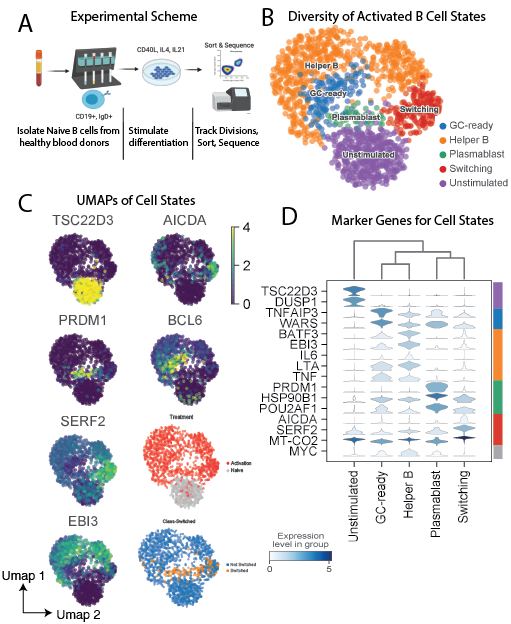
\includegraphics[width=8cm, keepaspectratio]{figs/prelim_paper2/BCellLineagePaper_Figure 1.png}
\caption[Experimental overview and transcriptional data for Naive B cell activation].{(A) Experimental Scheme (B) Annoated UMAP of the identified transcriptional states (C) UMAPs of marker gene expression levels and inferred CSR status. (D) Violin plots of marker genes for each cell state}
\label{fig:paper2_prelimfig_1}
\end{figure}

\begin{figure}[htb!]
\centering
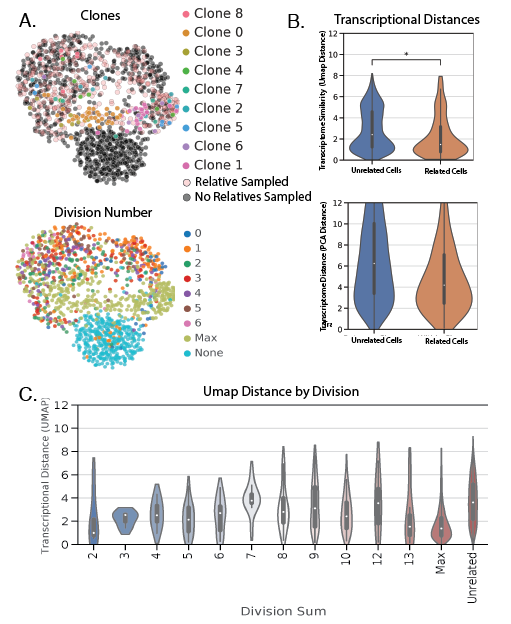
\includegraphics[width=8cm, keepaspectratio]{figs/prelim_paper2/BCellLineagePaper_Figure 2.png}
\caption[Transcriptomic similarity of clones \textit{in vitro}]{(A) UMAP projection showing the largest clones in the dataset (top) and the dye tracking division number of each clone (bottom) (B) Transcriptional distances between related and unrelated cells in UMAP (top) and PCA (bottom) space. p$<$0.01 by Kolmogorov-Smirnov test (C) UMAP distance plotted by division sum (2 divsions are siblings, 4 divisions are cousins, etc) of the related pairs of observed cells}
\label{fig:paper2_prelimfig_2}
\end{figure}

\begin{figure}[hbt!]
\centering
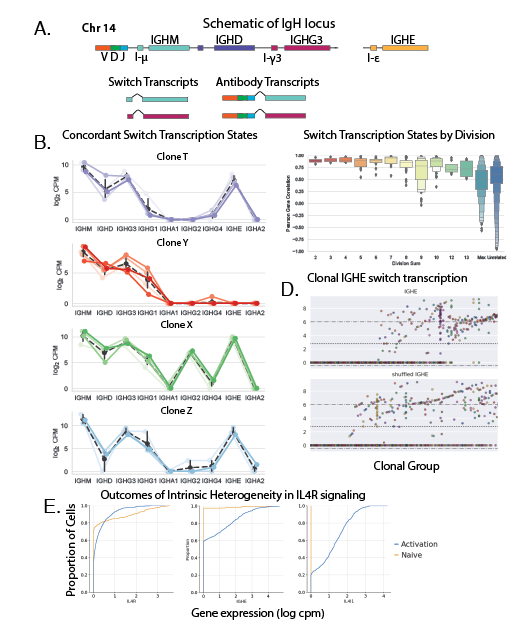
\includegraphics[width=14cm, keepaspectratio]{figs/prelim_paper2/BCellLineagePaper_Figure 3.png}
\caption[Concordant Switch Transcription States amongst related cells]{(A) A schematic of the IgH locus and switch transcription (B) Point plots showing diverse yet concordant switch transcription states amongst clonal groups (C) Boxen plot showing concordance in switch transcription state decreased over division-time (D) Cascade plot showing clonal effects in IGHE transcription levels}
\label{fig:paper2_prelimfig_3}
\end{figure}


%%%%%%%%%%%%%
%% Paper 2 %%
%%%%%%%%%%%%%

\begin{figure}[hbt!]
\centering
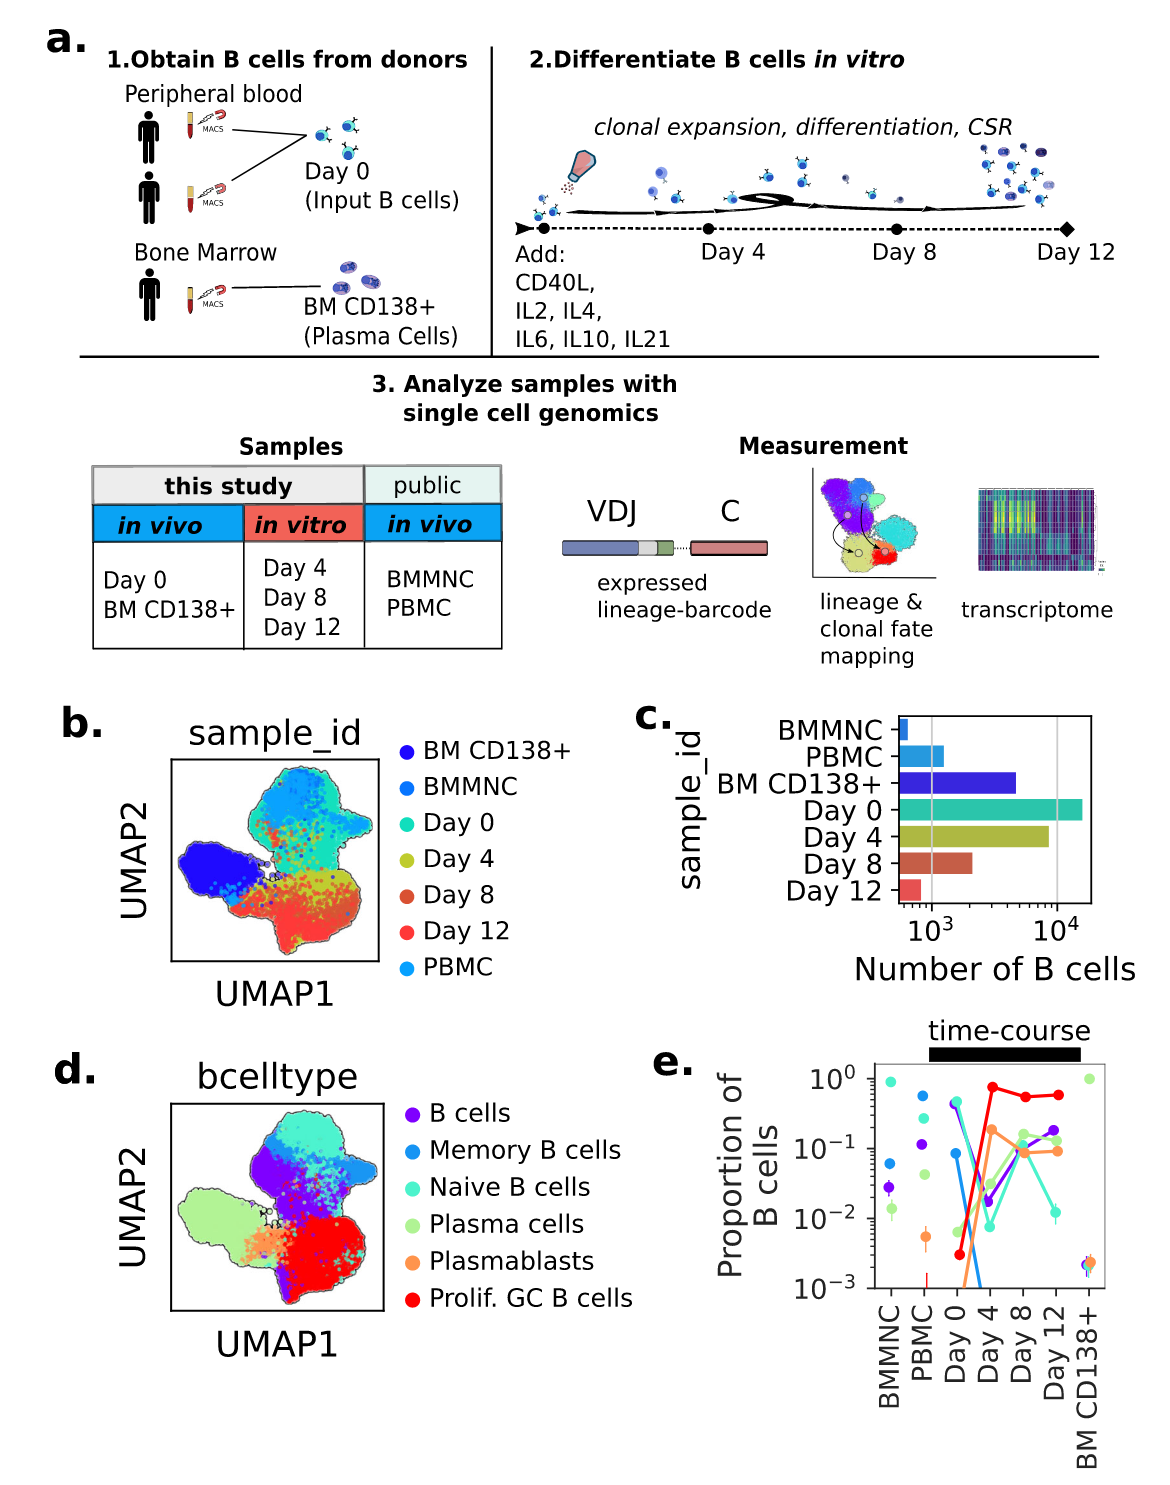
\includegraphics[width=12cm, keepaspectratio]{figs/paper2/fig1_bcd.png}
\caption[Experimental overview for studying \textit{in vitro} B cell dynamics using integrated single-cell genomics and lineage tracing.]{(1) B cells or Plasma cells purified from blood or bone marrow using MACS. (2) B cells from the same purification stimulated with the StemCell B cell Expansion kit. \textit{in vitro} differentiation samples collected on days 4, 8, and 12. (3) Single-cell genomic data collected and analyzed schematic. (B) UMAP embedding separate cells into distinct clusters, with dots as cells colored by sample origin. (B, C) Countplot of B cells passing QC for each sample (colors same as (B)). (D) UMAP embedding with cell type annotations. (E) Proportion of B cell types in each sample. Time course samples are connected by lines. Error bars represent 95 percentile intervals calculated by resampling.}
\label{fig:paper2_fig_1}
\end{figure}

\begin{figure}[hbt!]
\centering
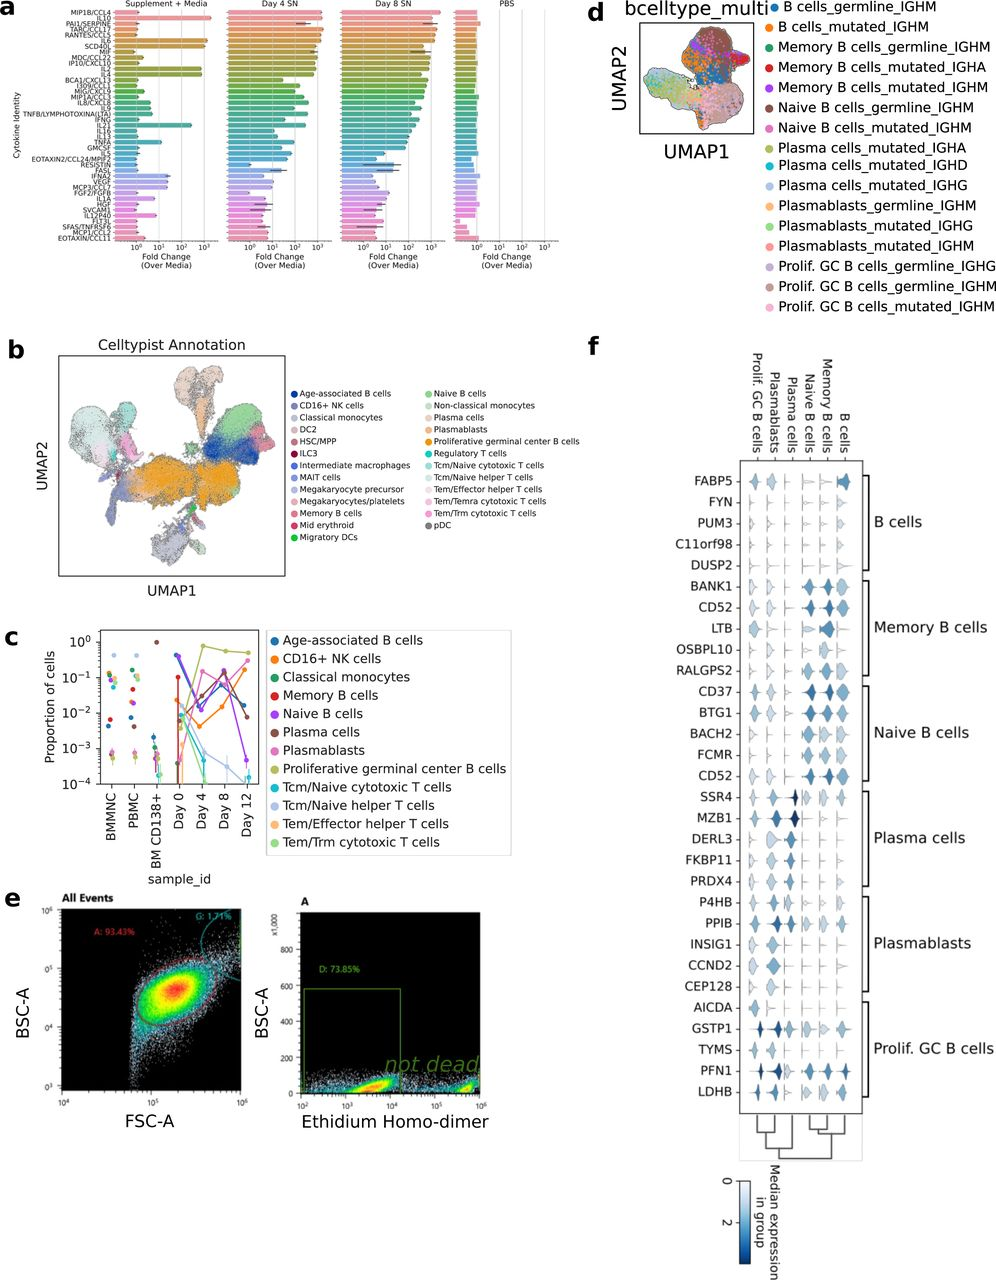
\includegraphics[width=14cm, keepaspectratio]{figs/paper2/figs1_bcd.jpg}
\caption[Analysis of stimulation cocktail and presentation of pre-processing steps.]{(A) Identities and relative abundance over the media of a panel of 80 human cytokines. Cytokines with fold change $>$ 2 are shown. SN, supernatant. PBS, Phosphate Buffered Saline. (B) UMAPs of all cells in the dataset, colored as shown in legends. The Celltypist-generated labels were kept for downstream analysis, except “Age-associated B cells” were changed to “B cells.” (C) UMAPs colored by multi-modal labeling of B cells. (D) Pointplot quantifying the proportion of celltypes in each sample\_id. (E) Scatter plots of representative FACS data. (F) Top differentially expressed genes between cell types}
\label{fig:paper2_fig_s1}
\end{figure}

\begin{figure}[hbt!]
\centering
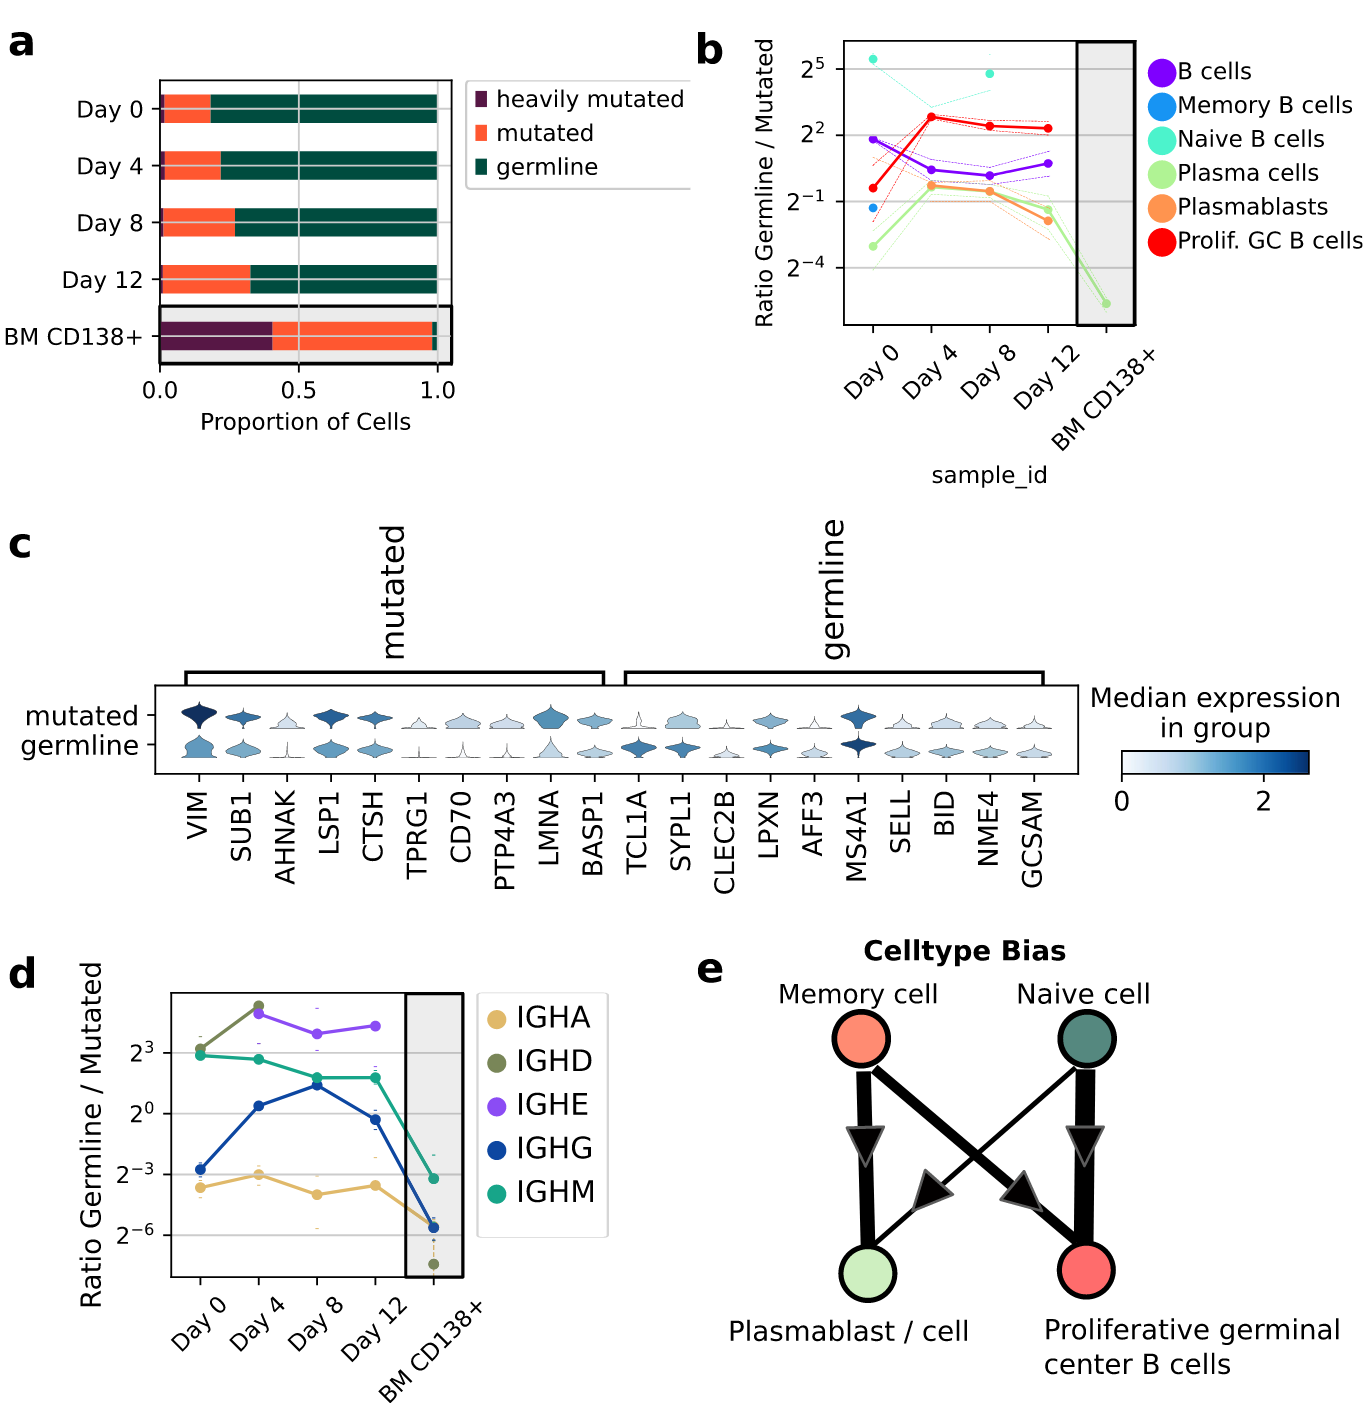
\includegraphics[width=14cm, keepaspectratio]{figs/paper2/fig2_bcd.png}
\caption[Characterization of cell-intrinsic phenotypes using VDJ mutation status.]{(A) Proportion of germline, mutated, and heavily mutated B cells in the samples; gray boxes illustrate BM CD138+ which is not part of the time course but serves as a comparison sample. (B) Ratio of germline to mutated cells in each cell state over the time course. (C) Top differentially expressed genes in between mutation categories in Proliferative germinal center B cells. Gene expression is log base 2 umis per 10,000. (D) Ratio of germline to mutated cells for each isotype group. Gray box as in (A). (B, E) Illustration of the inferred cell-type biases from (B). Error bars in all figures are 95 perecentile confidence intervals calculated by resampling.}
\label{fig:paper2_fig_2}
\end{figure}


\begin{figure}[hbt!]
\centering
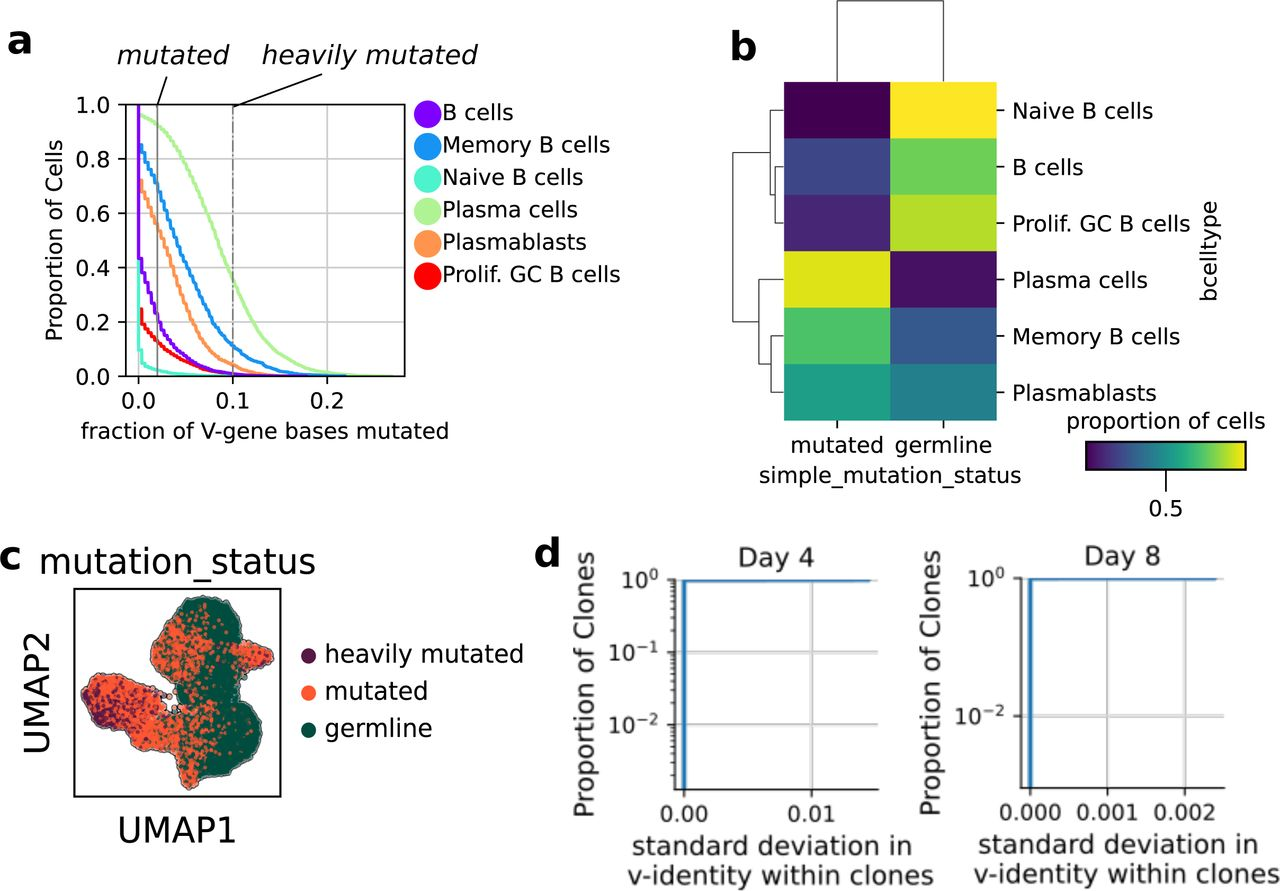
\includegraphics[width=14cm, keepaspectratio]{figs/paper2/figs2_bcd.jpg}
\caption[Validation of population based lineage inference.]{(A) Empirical cumulative distributions of the fraction of V-gene based mutated away from the germline V-gene, for each transcriptomically defined B cell type. (A, B) Heat map (confusion matrix) showing concordance between the mutation status based on (A) and each B cell type label based on Leiden clustering. (A, C) UMAP plot colored by the mutation status assigned based on (A). (D) Empirical cumulative distributions of the SD in V-identity within clones showing mutations are not collected within the V-genes of clones over the time course.}
\label{fig:paper2_fig_s2}
\end{figure}

\begin{figure}[hbt!]
\centering
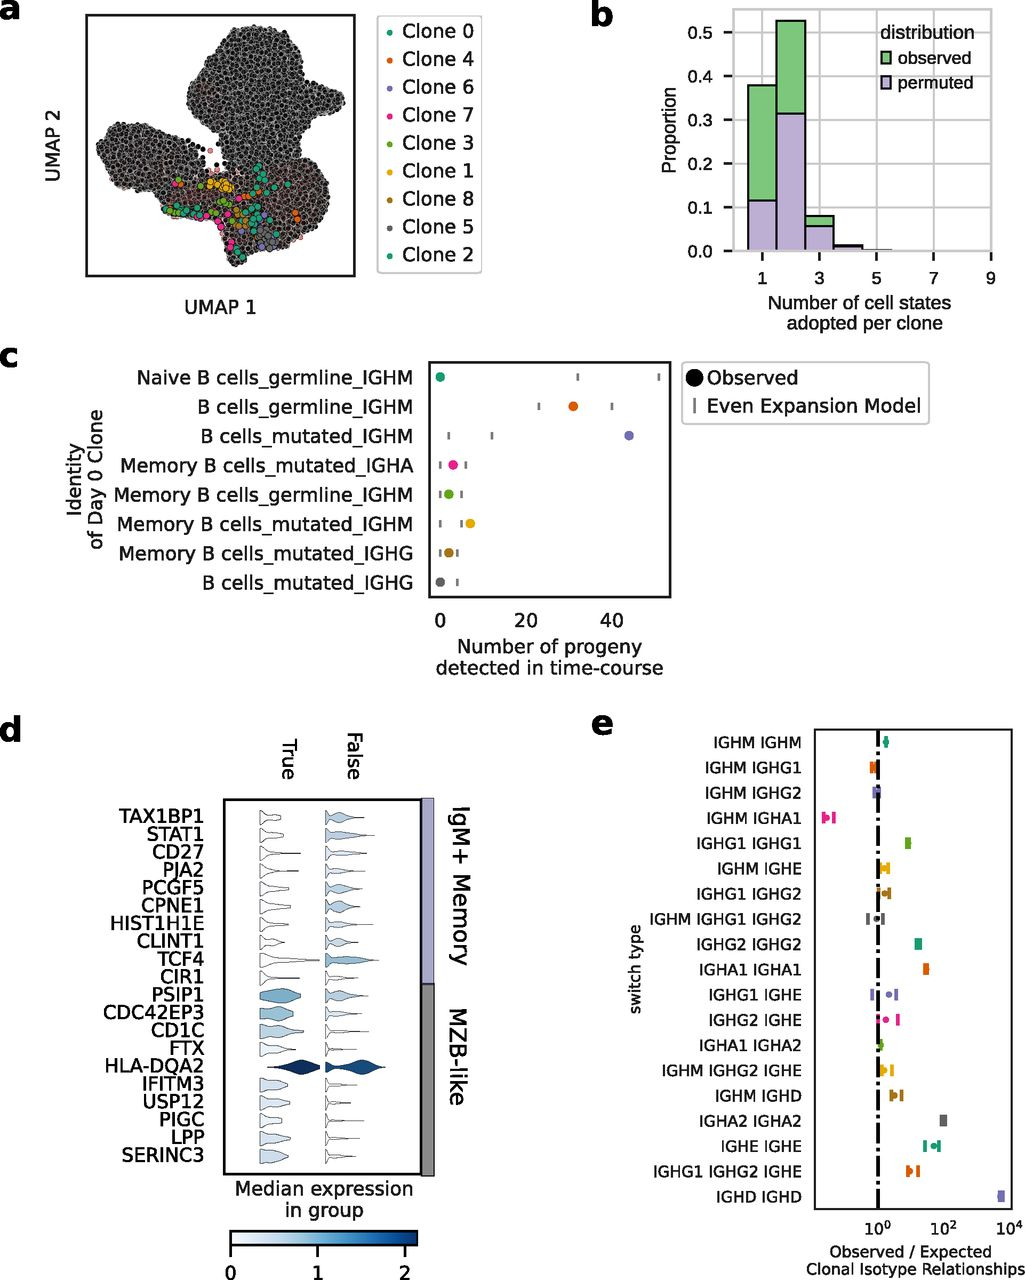
\includegraphics[width=14cm, keepaspectratio]{figs/paper2/fig3_bcd.jpg}
\caption[Clonal families allow inference of intrinsic proliferative ability, limited clonal fate outcomes, map of class-switching \textit{in vitro}.]{(A) UMAP embedding displays the largest clonal families detected. (B) Stacked histogram compares cell fate outcomes within clones to permuted clonal labels, with permutation restricted within respective mutational groups to analyze intrinsic bias not explainable by mutation status. (C) B cells with mutated IGHM BCRs show over-representation in the differentiated population. Observed data contrasted with a model where Day 0 clonal structure expands evenly for eight divisions and is randomly resampled. (D) Differential expression analysis between persistent and non-persistent clones in mutated IGHM B cell population. (E) Observed-to-expected clonal isotype relationship ratio for detected clonal isotype relationships.}
\label{fig:paper2_fig_3}
\end{figure}

\begin{figure}[hbt!]
\centering
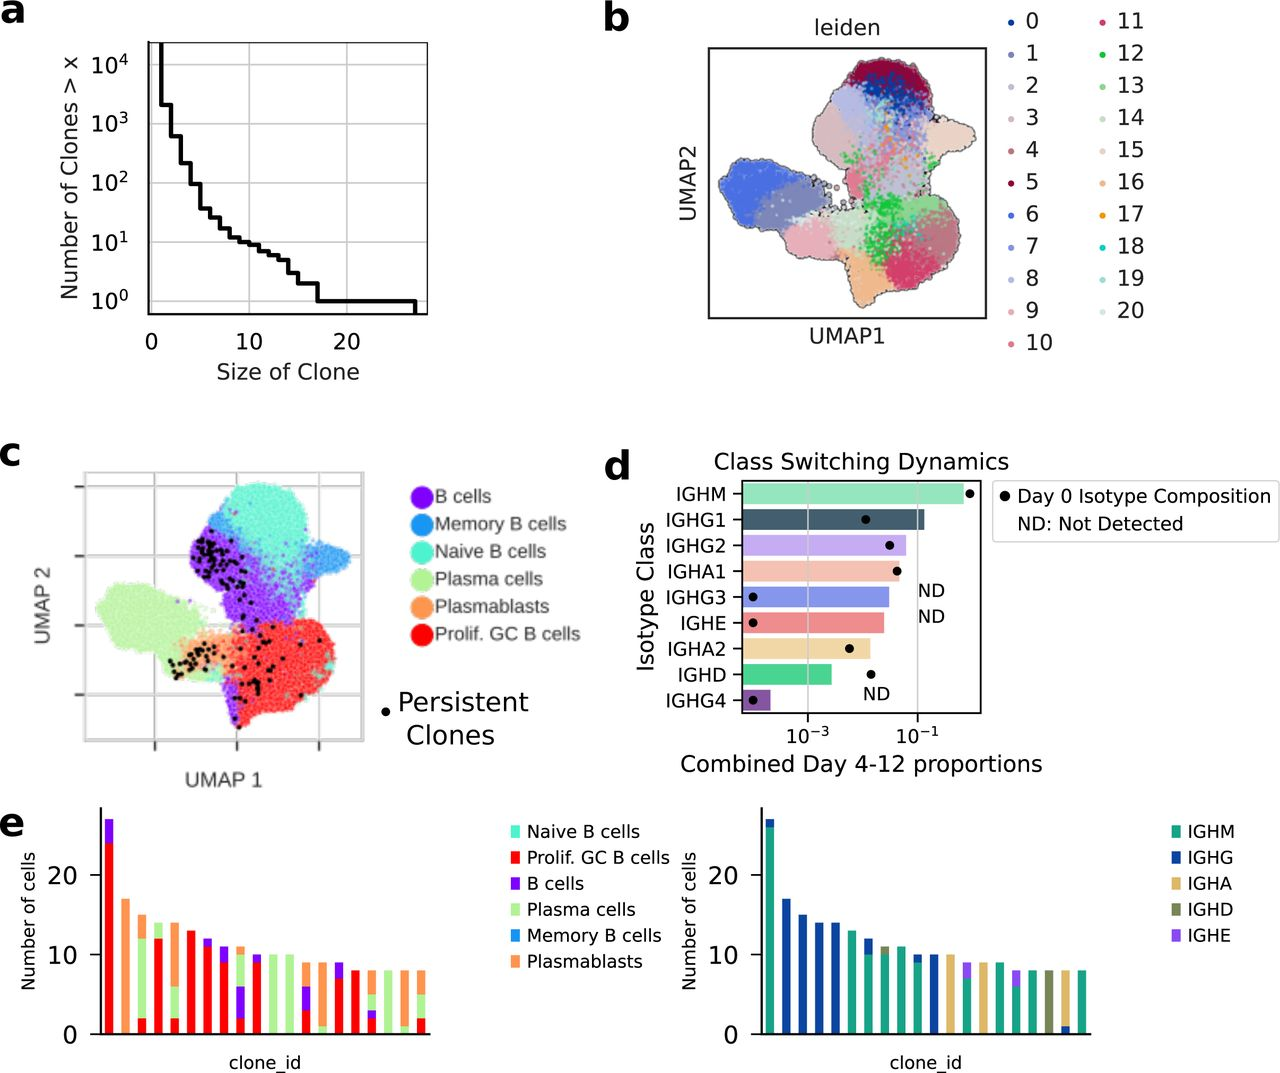
\includegraphics[width=14cm, keepaspectratio]{figs/paper2/figs3_bcd.jpg}
\caption[Clonal analysis of cell identity outcomes.]{(A) Clone size distribution of the B cell population from the \textit{in vitro} time course. (B) UMAP showing results of the Leiden clustering used for clonal fate bias calculations. (C) UMAP showing all cells from persistent clones in black. Persistent clones are clones detected at multiple time points. (D) Class-switching (isotype) dynamics during the culture. ND, not detected in the Day 0 population, a pseudo-count of 1 is added for visualization purposes. (E) Countplots of the largest clones detected and their transcriptomically defined cell fates and amplicon sequencing defined isotype status.}
\label{fig:paper2_fig_s3}
\end{figure}

\begin{figure}[hbt!]
\centering
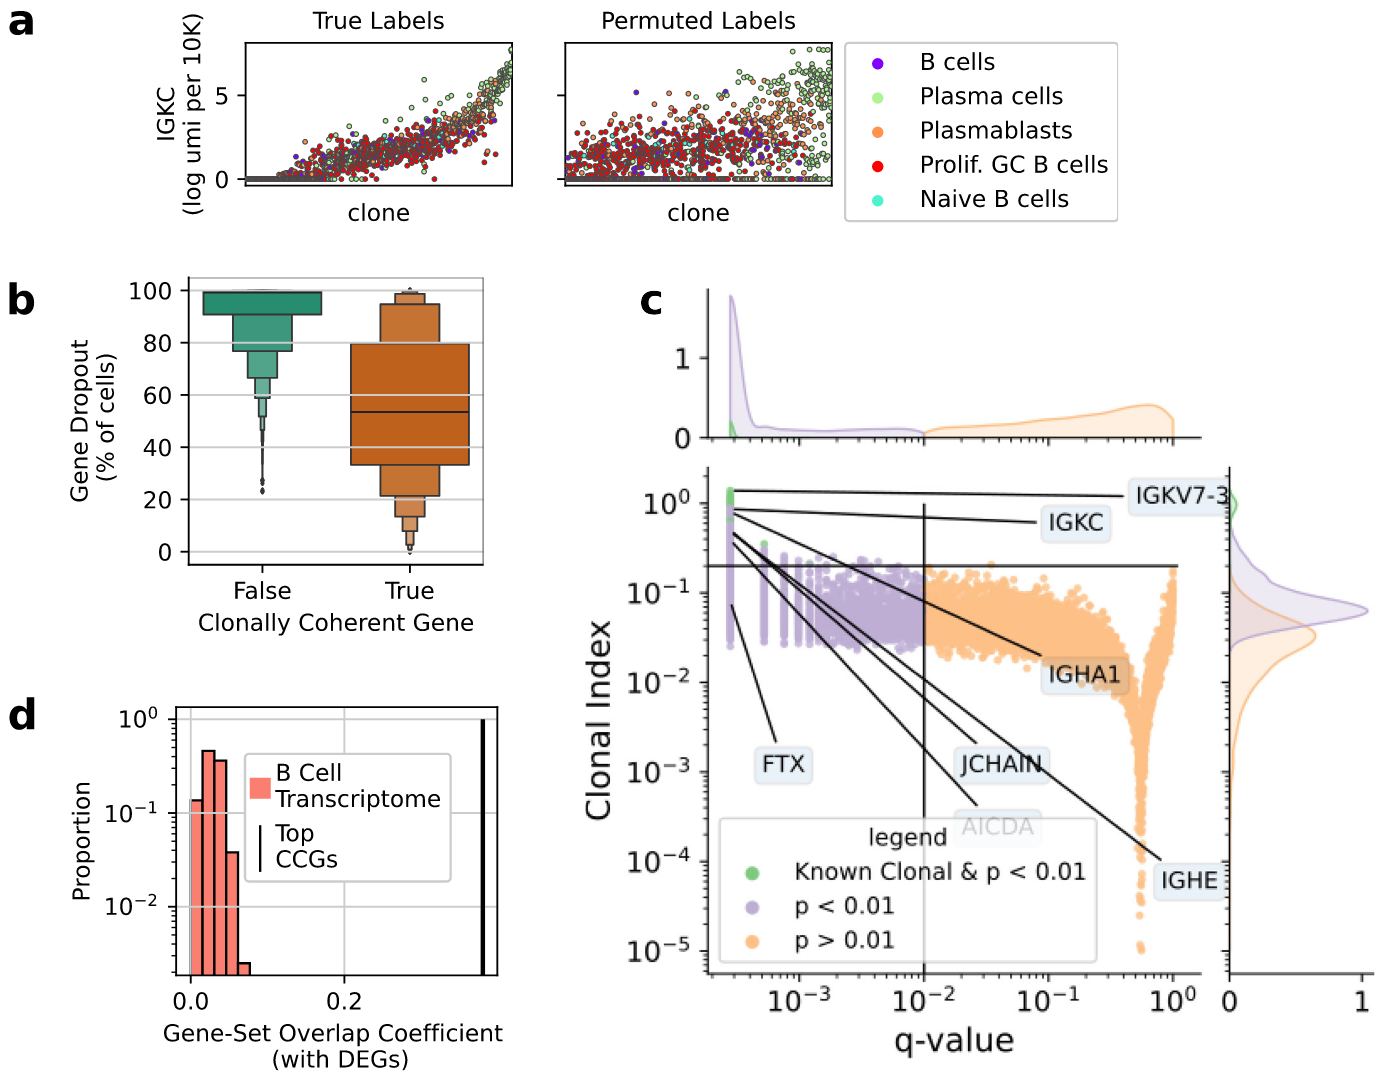
\includegraphics[width=14cm, keepaspectratio]{figs/paper2/fig4_bcd.png}
\caption[Clonal transcriptional programs are strongly enriched for fate determining genes.]{(A) Prototypical cascade plots showing IGKC expression amongst IGKC+ clones determined via immune repertoire sequencing. Each column is a clonal family of size $\geq$ 4. Families are rank-ordered by the mean gene expression of the family. Each dot is a cell, colored by the cell state label. The true clonal families are plotted on the left and a permutation of the clonal labels is plotted on the right. (B) Boxen plot showing the distribution of \% dropout for all genes tested. Genes across the entire distribution of detection rates were detected as clonal genes. Genes not detected as clonal were often very lowly expressed. (C) A volcano plot showing results of the transcriptome-wide permutation test. Q values are the Benjamini–Hochberg–corrected P-values and the clonal index is a normalized metric of expression variance described in the Materials and Methods section. Genes of interest are labeled and groups of interest are colored. Known clonal genes are the variable immunoglobulin genes. (D) The set of top CCGs strongly overlap with the set of top cell state defining genes compared to sets of randomly selected genes (P < 0.001). The null expectation is the B cell transcriptome, which were size-matched sets of genes sampled randomly from the set of genes in at least 10 \% of B cells.}
\label{fig:paper2_fig_4}
\end{figure}


\begin{figure}[hbt!]
\centering
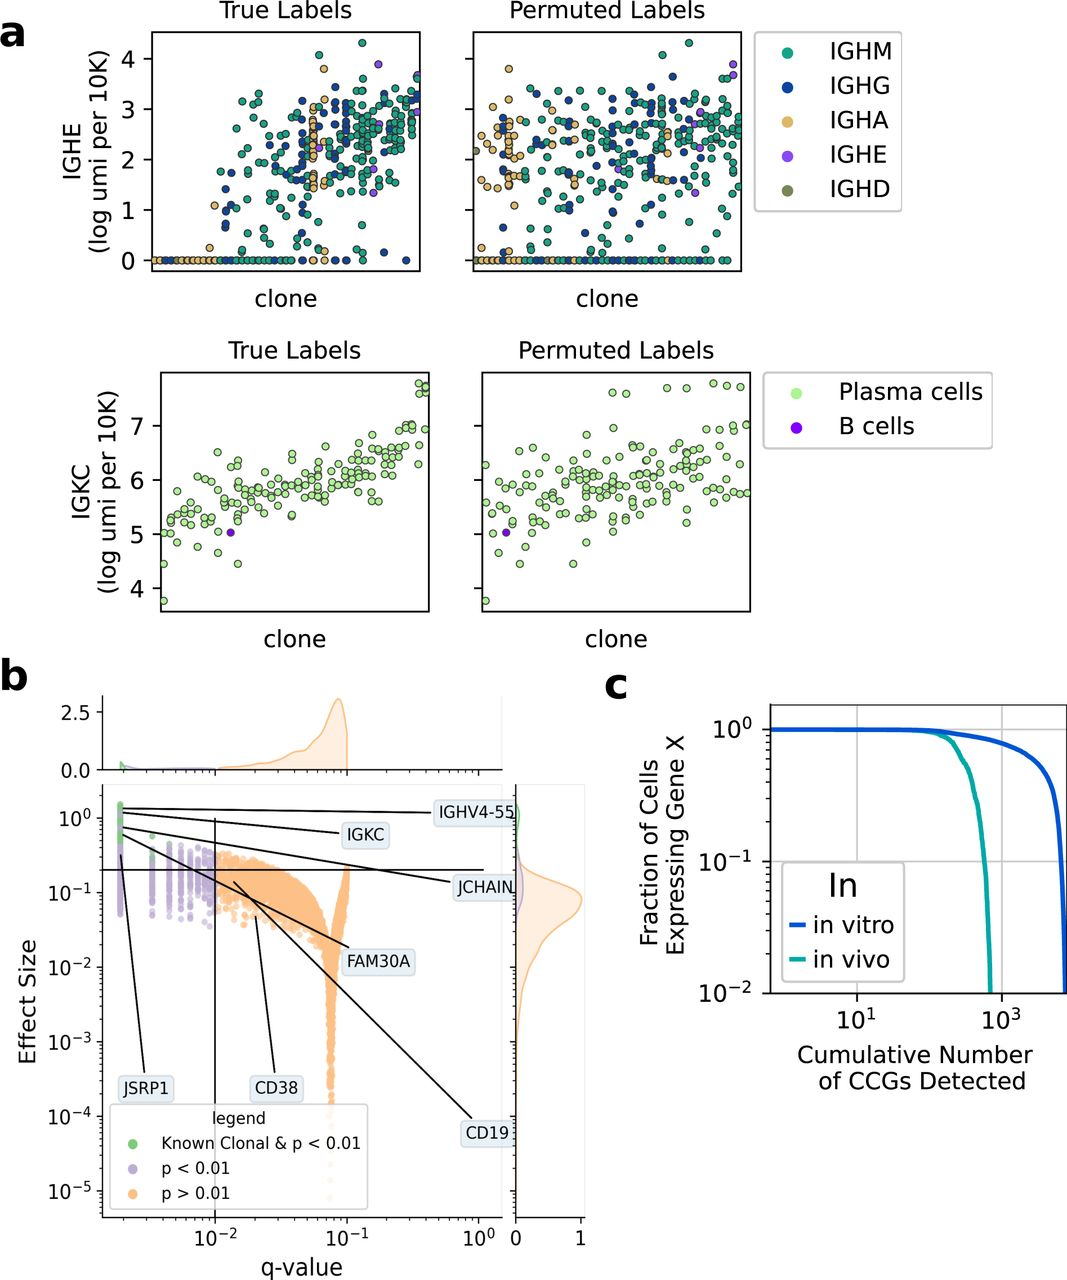
\includegraphics[width=13cm, keepaspectratio]{figs/paper2/figs4_bcd.jpg}
\caption[Analysis of persistent \textit{in vivo} transcriptional programs.]{(A) (Top) Cascade plot of IGHE expression in differentiating B cell clones, colored by the isotype associated with their VDJ sequence. (Bottom) Cascade plot of IGKC expression of IGKC+ clones in the bone marrow sample (B) A volcano plot showing results of the transcriptome-wide permutation test only for the \textit{in vivo} (BM CD138+) sample. The q-values are Benjamini–Hochberg–corrected and the clonal index is a normalized metric of expression variance described in the Materials and Methods. Genes of interest are labeled and groups of interest are colored. (C) ecdf plot of the number of clonal genes detected with a q-value $<$ 0.01 by the fraction of cells expressing a given gene (also known as \% gene dropout).}
\label{fig:paper2_fig_s4}
\end{figure}



% Full title as you would like it to appear on the page
\chapter{Mapping the Statistics of the human B cell repertoire}
% Short title that appears in the header of pages within the chapter
\chaptermark{Repertoire \textit{in vivo}}

\section{Abstract}
B cells generate pathogen-specific antibodies, which provide adaptive protection against infectious microbes. Unlike most proteins, antibodies are not genetically encoded at birth. Rather, they are stochastically generated and then modified in evolutionary processes acting on the B cell populations within an individual. These populations clonally expand, migrate, and home to long-term niches throughout the body, but the dynamics of differentiation, proliferation, and migration patterns in the human immune system remain mostly inferred from mouse studies. To address this, we sequenced the B cell receptors (BCRs) and transcriptomes at the single-cell level in multiple immune-rich tissues from six individuals. These paired data enabled us to examine the phenotypic patterns of expansion, migration, and differentiation of related B cells (lineages).

While most BCRs are detected in just a single tissue, we observed B cells with identical BCRs in multiple tissues. These cells differed from other subsets. They had often cycled recently and had more hypermutated BCRs than cells confined to a single tissue. Using phylogenetic approaches, we discovered that lineages often co-localize within the same tissue. However, when lineages reach a threshold size in the peripheral blood and secondary lymphatic organs (SLOs), their members are likely to be found in other tissues. This indicates that cellular migration from blood and SLOs is a probabilistic process in which cross-tissue sharing occurs when lineages attain sufficient size. Furthermore, we identified a hierarchy in migration patterns between tissues, with the spleen as the primary destination for hypermutated B cells and the bone marrow as the final location. Notably, the bone marrow had the largest fraction of private lineages compared to other examined tissues, consistent with its role as a terminal destination for plasma cells. Collectively, our findings elucidate the evolutionary landscape of B cell populations across tissues and show that the peripheral blood provides limited insights into the dynamics and composition of the human B cell repertoire.

\section{Introduction}
 Antibodies are developed by the immune system in response to pathogens and  provide protection to an individual in future exposures.  They are genetically encoded in B cells, which can remain alive throughout the lifetime of the individual\cite{slifka1998humoral}. These B cells provide long-term immune protection against previously encountered pathogens, as well as the capacity to rapidly respond to similar pathogens. During immune responses, clonal populations of B cells compete to receive proliferation and differentiation signals which direct them to become short or long-lived antibody secreting cells or memory B cells. 

Previous studies have uncovered much about the dynamics of this process in mice\cite{victora2022germinal},  and much is known about the characteristics of different B cell populations in humans\cite{halliley2015long, glass2020integrated, tarlinton2023making}, however, we still know very little about the statistics of B cell differentiation in healthy humans. As a result, it remains unclear, for instance, how the memory B cell subset in humans is related to the antibody secreting cell subset, or how the different types of antibody secreting cells are related to one another\cite{tarlinton2023making}. 

In principle, questions about the genetic relationships of different B cells can be resolved by sequencing the B cell receptor (BCR) of B cells in different subsets and investigating the phylogenetic relationships of the cells in these groups\cite{ellebedy2016defining,briney2019commonality,phad_lanza_2022clonal, horns2016lineage}. However, most effector B cells in humans reside in tissues that are difficult to sample, while previous BCR sequencing studies on healthy humans have largely been carried out on B cells sampled from the peripheral blood. To address this gap, several recent studies have surveyed B cell populations resident in other tissues\cite{glass2020integrated, tabula2022tabula, dominguez2022cross}.  These studies reveal that B cells living in other tissues are exist in a range of diverse effector states, which often differ from the B cell subsets that have been described in mice\cite{glass2020integrated, dominguez2022cross}. However, limitations in either the number of sampled B cells in these studies or the availability of the corresponding BCR sequences have made it impossible to use these studies to answer questions about the relationships between B cells in different tissues and states. Other work\cite{meng2017atlas, yang2021shared} revealed complex patterns of genetic relationships between the B cell populations sampled from a wide range of human organs by sequencing BCRs. However, these data lacked phenotypic information and single-cell resolution, making it difficult to interpret these relationships in light of the underlying cellular processes of differentiation and migration. 

Here we use a combination of single-cell transcriptome and BCR sequencing to simultaneously measure the phenotypic and genetic relationships of B cells resident in a range of immune-rich tissues in six healthy individuals. Our simultaneous measurement of the transcriptome and BCR allows us to associate BCRs with a B cell's functional state and to jointly investigate the patterns of B cell migration and differentiation between human organs.
\section{Results}

\subsection{The distribution of B cells in lymphatic tissues at rest}
 We obtained B cells from the vertebral bodies, supradiaphragmatic and mesenteric lymph nodes, spleen, and blood of 6 organ donors with no clinical history of cancer, immune disease, or active infectious disease at the time of death (Figure \ref{fig:study-overview}\textbf{a}, \ref{tab:donor-metadata}, methods). We used high-throughput droplet-based single cell RNA-sequencing to analyze the transcriptomes and BCRs of over 200 thousand single B cells. To increase the depth of BCR sampling, and to provide replication of the sampling and measurement process, we used the same platform to sequence only the BCRs of an additional 400 thousand B cells. 

Overall, we observe a remarkably quiescent immune system, with very few activated B cells detected in all donors (Figure \ref{fig:study-overview}\textbf{b}). A small fraction of all B cells (1-6\% per donor) appear to be actively proliferating as evidenced by the expression of M-phase markers such as MKI67 (methods, \ref{ED:cycling}).  Proliferating cells predominantly have an antibody secreting cell (ASC) phenotype, though we sampled a small number of proliferating germinal center B cells, as well as a small fraction of age-associated B cells (ABCs) that appear to be actively dividing (Figure \ref{ED:cycling}\textbf{d}).

\subsection{Distribution of cell types among organs}
The fraction of cycling B cells and B cell types in general was similar across tissues. However, the SLOs had a much larger relative abundance of memory B cells, which was offset by a smaller relative abundance of naive B cells (Figure \ref{fig:study-overview}\textbf{c}). Similarly, the the bone marrow had a much larger relative abundance of antibody secreting cells, offset by a smaller relative abundance of memory B cells. Cells with a germinal center-like phenotype were almost exclusively detected in SLOs, and at relative abundances near 1 in 1000, showing very limited ongoing systemic immune responses in all donors  (Figure \ref{fig:study-overview}\textbf{c}). Though the distribution of hypermutation levels in all  non-naive cell types was broad, we observed large differences in median hypermutation levels between antibody secreting cells and memory B cells, with ASC having median 10 additional mutations compared memory B cells in the same tissue\ref{fig:asc-overview}\textbf{d},\ref{ED:memoryb-overview}\textbf{d}).   
\begin{figure}
    \centering
    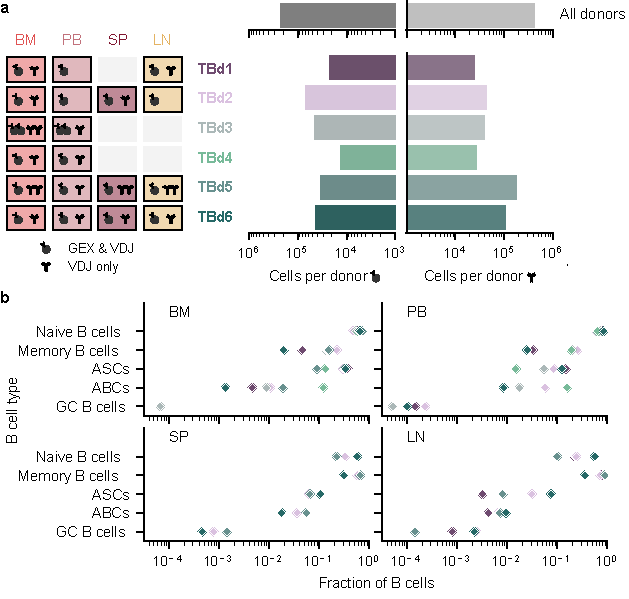
\includegraphics[width=10cm]{figs/Tabula_Bursa/Figure1_ab_antibody_version.pdf}

    \caption[\textit{In vivo} study overview]{Heterogeneity in antibody secreting cells (ASCs). (a) Low-dimensional (UMAP) representation of transcriptional heterogeneity in ASCs. Celltypist labels (top), and transcriptome-derived labels (bottom). Inset shows UMAP representation when cell-cycle associated genes are removed. (b) Genes distinguishing between the subtypes of ASCs, where the top half of the plot shows canonical genes often used for flow cytometry and the bottom shows the data-derived, transcriptionally detected genes which distinguish the subtypes. (c) The relative fractional abundance of ASC subtypes in different tissues averaged across all donors. (d) The distributions of  hypermutation levels (d),  and constant region usage (e) of the ASC subtypes}
    \label{fig:study-overview}
\end{figure}

\begin{table}[t]
\centering
\begin{tabular}{|c|c|c|c|c|}
\hline
\textbf{Donor} & \textbf{Age} & \textbf{Sex} & \textbf{Ethnicity} & \textbf{CoD} \\
\hline
TBd1 & 46 & F & Asian/J & CV stroke \\
TBd2 & 35 & M & AI/AN & Anoxia \\
TBd3 & 25 & F & Hisp/Lat & Head Trauma \\
TBd4 & 43 & F & Hisp/Lat & Anoxia \\
TBd5 & 45 & F & Asian/Fil & CV stroke  \\
TBd6 & 60 & M & Asian/Fil & Anoxia, cardiac arrest \\
\hline
\end{tabular}
    \caption[Demographic characteristics of donors]{Demographic characteristics of donors. "CoD" stands for "Cause of Death", "CV stroke" stands for "Cerebrovascular stroke", "Asian/J" stands for "Asian/Japanese", "AI/AN" stands for "American Indian or Alaska Native", "Hisp/Lat" stands for "Hispanic/Latino", and "Asian/Fil" stands for "Asian/Filipino"}
    \label{tab:donor-metadata}
\end{table}



\subsection{Phenotypic variability among memory and antibody secreting cells}



Initially, we automatically annotated the B cell types using an algorithm called \verb|celltypist|\cite{dominguez2022cross}. However, our data reveal substantial additional phenotypic variability within non-naive B cell subsets (Figures \ref{fig:asc-overview}, \ref{ED:memoryb-overview}). Among antibody secreting cells (ASC) (Figure \ref{fig:asc-overview}\textbf{a}), the variability was consistent with a prevailing understanding these cells have substantial phenotypic variation in mice and human (\cite{tarlinton2023making, halliley2015long}). 

\begin{figure}
    \centering
    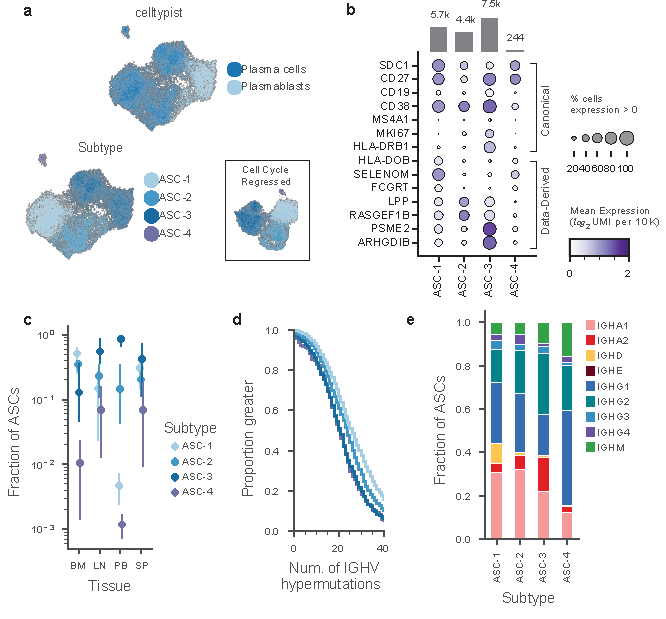
\includegraphics[width=12cm]{figs/Tabula_Bursa/Figure2_ASC_subtypes.pdf}

    \caption[Heterogeneity in antibody secreting cells (ASCs)]{ (a) Low-dimensional (UMAP) representation of transcriptional heterogeneity in ASCs. Celltypist labels (top), and transcriptome-derived labels (bottom). Inset shows UMAP representation when cell-cycle associated genes are removed. (b) Genes distinguishing between the subtypes of ASCs, where the top half of the plot shows canonical genes often used for flow cytometry and the bottom shows the data-derived, transcriptionally detected genes which distinguish the subtypes. (c) The relative fractional abundance of ASC subtypes in different tissues averaged across all donors. (d) The distributions of  hypermutation levels (d),  and constant region usage (e) of the ASC subtypes}
    \label{fig:asc-overview}
\end{figure}
There were four distinguishable types of ASC, which we label ASC-1 through ASC-4. A substantial fraction of ASC-3 were proliferating, had a gene expression signature that closely resembles previous descriptions of plasmablasts. For example, they expressed HLA molecules higher than other subsets (Figure \ref{fig:asc-overview}\textbf{b})\cite{sanz2019challenges}. Notably, nearly half of ASC-3 have no detectable M-phase markers, but have otherwise indistinguishable gene expression profiles from cycling ASC-3, suggesting that these cells have recently stopped cycling (Figure \ref{fig:asc-overview}\textbf{a}). Specifically, regressing the expression of the proliferation marker MKI67 collapses the distinction between the gene expression space of cycling and non-cycling ASC-3 (Figure \ref{fig:asc-overview}\textbf{a} inset). The other types of ASCs appeared non-proliferative, were commonly found outside the peripheral blood, and had gene expression consistent with long-lived plasma cell subtypes\cite{sanz2019challenges}(Figure \ref{fig:asc-overview}\textbf{b}). In particular, ASC-1 are primarily resident in the bone marrow and have the canonical markers of long-lived plasma cells (\cite{halliley2015long} (Figure \ref{fig:asc-overview}\textbf{b,c}). ASC-4 is strongly enriched in the SLOs, but transcriptionally similar to ASC-1. We performed differential expression analysis on these subsets of ASCs and found that ASC-1 and ASC-4 had higher expression of FCGRT (FcRN), SELENOM, and HLA-DO than other subsets. (Figure \ref{fig:asc-overview}\textbf{b}. SELENOM may participate in disulfide bond creation, but has no described role in antibody secretion or plasma cell longevity. We detected plasma cells of all isotypes, including a small proportion of plasma cells which were IGHD+ and heavily hypermutated compared to other isotypes (Figure \ref{fig:asc-overview}\textbf{d}). With respect to the memory B cells, we characterized their phenotypic profiles in a similar manner (Figure \ref{ED:memoryb-overview}) and found results generally consistent with a multi-omic characterization of B cells made by\cite{glass2020integrated}.

\subsection{VDJ sequencing reveals sharing of a subset of expanded clones}
\begin{figure}
    \centering
    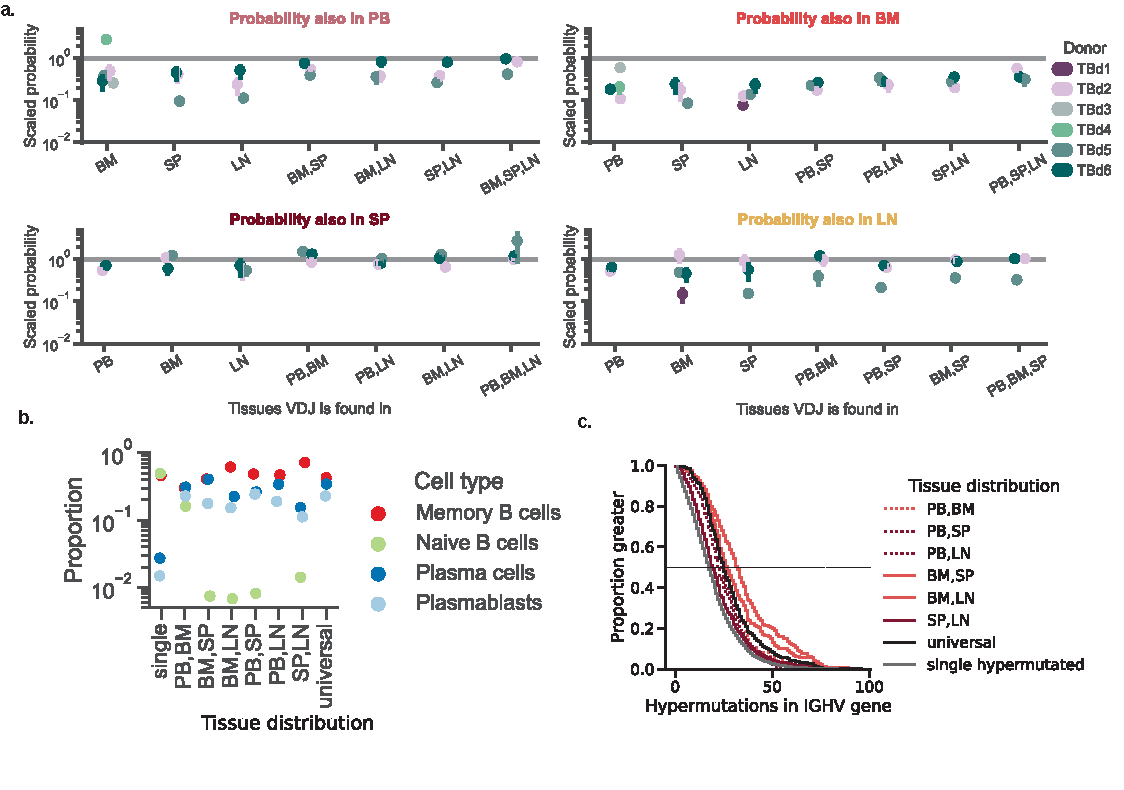
\includegraphics[width=10cm, keepaspectratio]{figs/Tabula_Bursa/Figure3_revised.pdf}
    \caption[Characteristics of clonally expanded B cells.]{ (a) Probability that a B cell is found in an additional tissue, given it is found to be expanded in one or more other tissues. (b) Fractional abundances, and (c) the distribution of hypermutation levels of B cells as a function of the tissues their heavy chain antibody sequences were found in.}
    \label{fig:clonally-expanded-B-cells}
\end{figure}
 In all samples, we sequenced the transcripts encoding for the heavy and light chains of the BCR, which we used to reveal the clonal relationships between B cells residing in different organs (methods, SI). We find that the probability of sampling identical nucleotide heavy chain sequences in different donors is vanishingly rare: after identifying and removing rare cross-contamination events (SI), we find only 5 of more than 600 thousand unique VDJs shared between donors, (Figure \ref{ED:multidonor-vdjs}A). This observation is consistent with earlier work which showed convergent VDJ recombination is an extremely rare event (\cite{mora2019many, briney2019commonality}). Thus, we interpret the nucleotide sequence of the heavy chain variable region as a unique clonal identifier of B cells (SI). 
 
\begin{figure}
    \centering
    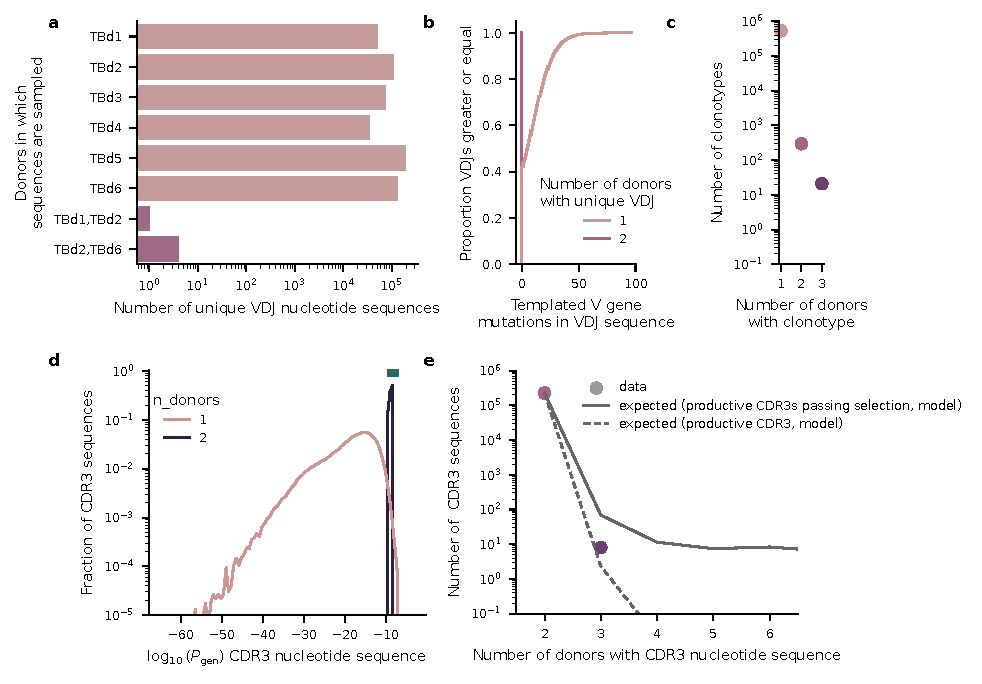
\includegraphics[width=10cm]{figs/Tabula_Bursa/ED_donor_sharing.pdf}
    \caption[Characteristics of  VDJ sequences found in multiple donors.]{(a) Number of unique nucleotide VDJ sequences as a function of the donors they were found in. (b) Distribution of the number of hypermutations in the templated portion of the IGHV gene as a function of the number of donors a VDJ sequence was found in. (c) Number of shared "clonotypes" in our data, where a clonotype is taken to be a sequence with an identical germline V gene, J gene, and CDR3 amino acid sequence. (d) Recombination probabilities for the CDR3 nucleotide sequence as a function of the number of donors the CDR3 was found in. Green dashes denote the CDR3's associated with the VDJ sequences shared between multiple donors. (e) Number of shared CDR3s in our data compared to the number expected under given the overall distribution of recombination probabilities shown in (d). The two models are described in detail in the SI.}
    \label{ED:multidonor-vdjs}
\end{figure}

Consistent with the variation in cell states revealed by our gene expression data, the characteristics of the VDJs differ between the tissues. In all donors, the peripheral blood and the bone marrow contain a substantial fraction of unhypermutated VDJs, while the bone marrow is also the site with the most heavily hypermutated sequences. Consistent with the relative paucity of naive B cells in the SLOs, VDJs sampled from these tissues predominantly contain hypermutations. 

Because we have single cell information, we are able to find that clonal expansion without hypermutation is a relatively common event: in all samples, about 1 in 100 of all unique VDJ sequences are identical in multiple cells. Though evidence of clonal expansion can be found among cells of all types, it is particularly prominent among antibody secreting cells, especially Type 3 ASCs, whether or not they are actively expressing M-phase associated genes. 

Next, we quantified the rates of clonally expanded VDJ sharing between tissues. To account for limited sampling, we derive a scaled probability estimate that makes use of technical replicates of tissue samples (Figure\ref{fig:clonally-expanded-B-cells}\textbf{a}). VDJs expanded in one tissue are found in others with probabilities often exceeding 0.1. The patterns of relative sharing suggest a hierarchy between the lymphatic organs organs: the probability that a VDJ expanded in a given organ is also present in the spleen is often indistinguishable from 100\%, whereas the probability that it is found in the peripheral blood or in the bone marrow is typically lower. Finally, the probability of encountering a VDJ in any given tissue increases with the number of other tissues it has been n in (Figure \ref{fig:clonally-expanded-B-cells}\textbf{a}). Multi-tissue-VDJs were enriched for the antibody secreting cell and memory B cell phenotypes  (Figure \ref{fig:clonally-expanded-B-cells}\textbf{b}). Furthermore, these VDJs are more strongly hypermutated than the comparable VDJs from ASCs and memory B cells restricted to a single tissue (Figure \ref{fig:clonally-expanded-B-cells}\textbf{c}). Finally, our data do not exclude the possibility that all cycling cells are shared between at least a pair of organs but we emphasize that not all cells that are shared are cycling: cells without M-phase markers account for a substantial fraction of all shared cells (Figure \ref{ED:cycling}).


\subsection{The distribution of related B cells among lymphatic tissues}
\begin{figure}
    \centering
    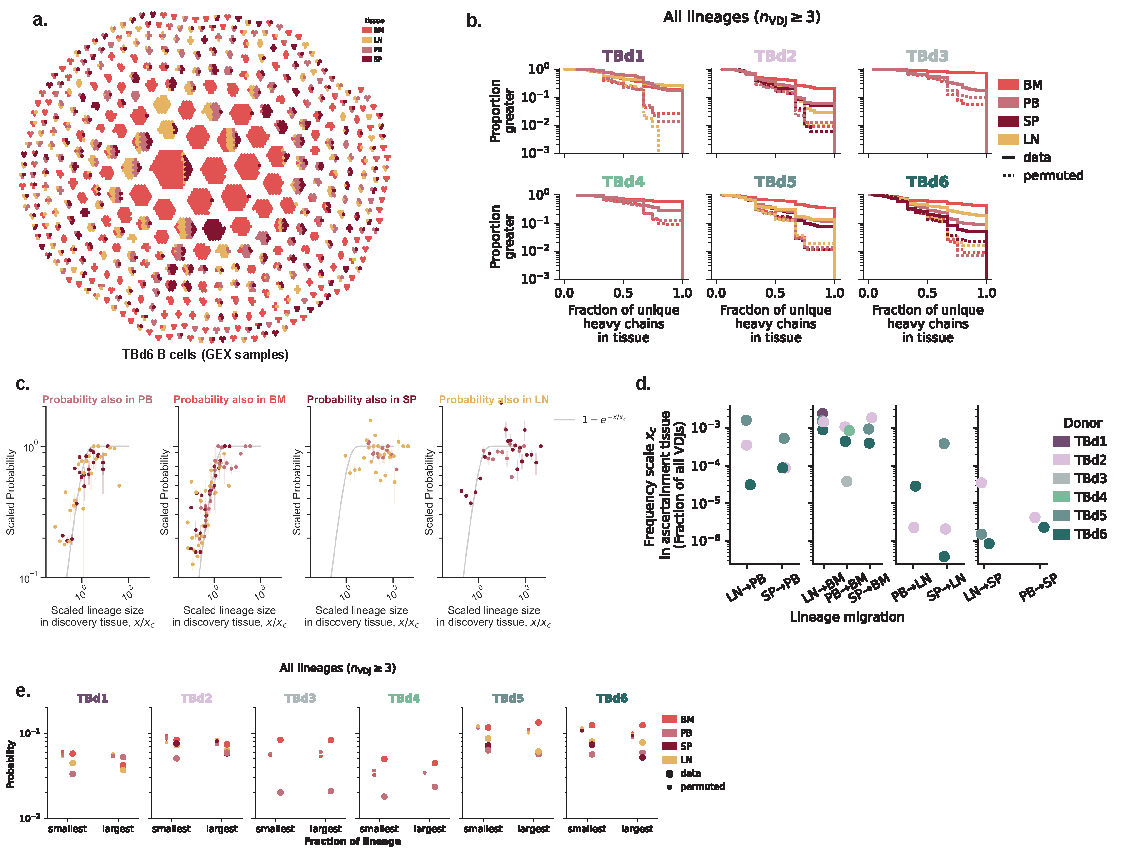
\includegraphics[width=10cm, keepaspectratio]{figs/Tabula_Bursa/Figure4_revised.pdf}
    \caption[Tissue distribution of phylogenetically related B cell, or lineages.]{(a) A representation of the tissue composition of lineages. Each hexagon denotes a cell, and each connected group of hexagons represents a lineage. Cells are colored by the tissue they were sampled in. Each tissue has been down-sampled to the same overall number of cells. (b) The distribution of the fraction of unique VDJs in the lineage found in a certain tissue. Dotted lines denote the distributions obtained after a random permutation of the tissue labels among the sampled cells.  (c) The probability that a lineage is discovered in a tissue, as a function of the total size of that lineage in another, ascertainment, tissue. Points are colored by ascertainment tissue, and each panel corresponds to a different discovery tissue. Size represents the total fraction of unique heavy chain sequences attributable to the lineage, and is scaled by a single parameter, the critical size $x_c$. (d) The critical size of a lineage in the ascertainment tissue used to scale lineage sizes in (c). (e) The probability that a tissue either contains the smallest or largest number of unique VDJ sequences in a lineage (relative to all other tissues). Large points are derived from the data, and small points represent a random permutation of the tissue labels among the sampled cells.}
    \label{fig:lineage-distribution}
\end{figure}

 B cells descended from the same VDJ recombination event carry a unique genetic recombination signature that we used to group B cells into clonal lineages. A striking feature of the distribution of lineages among the sampled tissues is the tendency for related cells to co-localize within the same tissue. (Figure \ref{fig:lineage-distribution}\textbf{a,b}). This co-localization is n in all tissues and in all donors except TBd1, and is particularly strong in the case of the bone marrow. (Figure \ref{fig:lineage-distribution}\textbf{b}).  However, we detect abundant sharing of large lineages between the sampled organs. This sharing follows a relatively simple pattern: conditional on sampling a lineage in the peripheral blood, the spleen, or a lymph node, the probability that lineage is present in a second tissue increases exponentially with its size (Figure \ref{fig:lineage-distribution}\textbf{c}). Lineages in the bone marrow deviate from this scaling: large lineages in the bone marrow are no more likely to be present in another tissue than smaller lineages detected in the bone marrow. This suggests that migration of B cells out of the peripheral blood, spleen, or bone marrow is governed by a relatively simple probabilistic process, where a small, but constant probability exists that a cell residing in one of these three tissues migrates to a new tissue. In contrast, we find little evidence of such a process in the bone marrow, which tends to be the most exclusive tissue, as evidenced by the fact that it is the tissue most likely to be both the minority and the majority location for a B cell lineage (Figure \ref{fig:lineage-distribution}\textbf{e}).

By examining the size at which lineages sampled in these three tissues are guaranteed to be n in another tissue, we uncover a hierarchy in the relative amounts of sharing between tissues. Lineages of relatively small size in the peripheral blood could be detected in the lymph nodes and spleen; lineages needed to reach a larger relative fraction in the spleen and lymph nodes to be also found in the blood, and an even higher size threshold was necessary for migration into the bone marrow (Figure \ref{fig:lineage-distribution}\textbf{d}). Overall, these patterns are consistent with the patterns of sharing of identical VDJs across tissues and suggest that the spleen in particular, and the lymph nodes to a lesser extent, may act as a first repository of B cells that have experienced affinity maturation, whereas the circulation of mature B cells in the peripheral blood, and finally localization in the bone marrow are less probable events.

%To understand the relative imbalance of lineage sharing amongst tissues, we calculated the number of times a specific tissue accounted for the smallest fraction and largest fraction of members in a lineage. Across all donors, these statistics deviated from a permuted null-expection for the bone marrow. 

\subsection{The distribution of tissues and cell types among groups of related cells}
 Overall, these results and the implied fractional abundance scales suggest that B cell migration is a relatively rare event relative to hypermutation. Given the differences in hypermutation rates of the same celltype in different tissues, we were interested in whether localization to certain tissues (e.g. the bone marrow) tended to occur deeper in lineage phylogenies. 

\begin{figure}
    \centering
    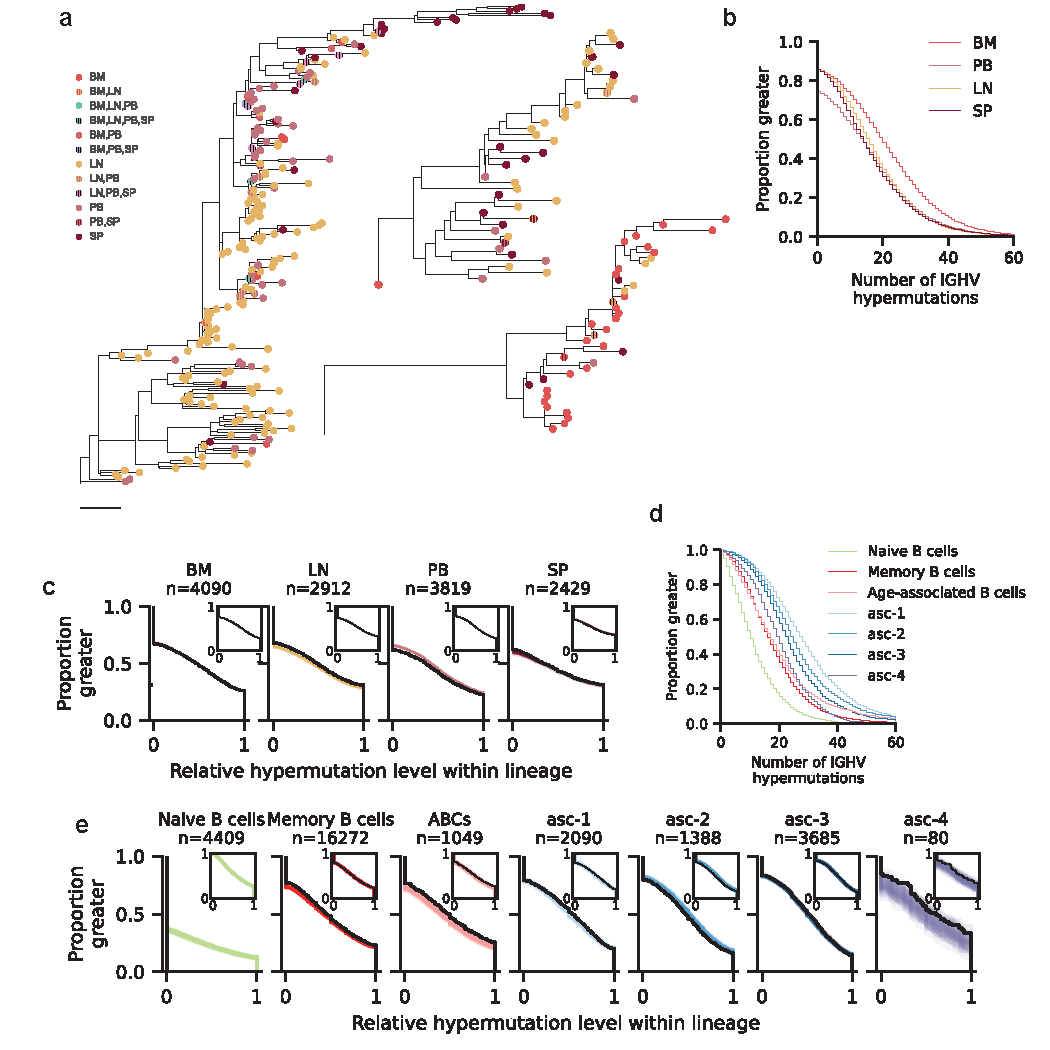
\includegraphics[width=10cm, keepaspectratio]{figs/Tabula_Bursa/Figure5_revised.pdf}
    \caption[Relationships between related cells.]{(a) Templated V gene trees depicting the relationships of B cells localized in different tissues in 3 example lineages from TBd6. Trees are rooted on the inferred germline V sequence. Leaves correspond to unique templated V sequences and are colored by localization. (b) The distribution of hypermutation levels of B cells belonging to lineages with membership in the indicated tissues. (c) Relative hypermutation levels of B cells within a lineage. In each panel, black lines denote the observed distribution in the data and the colored lines denote the 99\% confidence interval obtained by permuting tissue labels within lineages. On each panel, $n$ indicates the number of lineages among which the permutation was performed. Insets show the distributions with all cells with no templated V mutations excluded.  (d) The distribution of hypermutation levels of B cells belonging to lineages with any members in the indicated B cell subsets. (e) Same as (c), but for B cell subsets, rather than tissues. }

\label{fig:phylogenetic-relationships}
    
\end{figure}

This would cohere with the idea that affinity maturation occurs in other tissues such as the spleen or the lymph nodes before migration to the bone marrow. To investigate this, we compared the hypermutation level of cells residing in different tissues within lineages (Figure \ref{fig:phylogenetic-relationships}). Notably, the overall level of hypermutation varies not only between cells residing in different tissues, but also between their relatives: B cells in lineages with any members in the bone marrow are for instance also more hypermutated than comparable cells from the same tissue, even if they may not themselves reside in the bone marrow (Figure \ref{fig:phylogenetic-relationships}\textbf{b}). However, within lineages, cells located in different tissues were almost entirely uniformly distributed (Figure \ref{fig:phylogenetic-relationships}\textbf{c}), and are limited to the differential localization of naive B cells in different tissues. Once cells with no evidence of hypermutation in the templated V sequence are excluded, there remain no statistically significant differences between the measured distributions of hypermutation levels of related cells residing in different tissues (Figure \ref{fig:phylogenetic-relationships}\textbf{c}, insets).  An analogous observation can be made regarding the hypermutation levels of cells in different functional states. Despite systematic differences in the hypermutation levels of  different B cell subsets and their relatives (Figure \ref{fig:phylogenetic-relationships}\textbf{d}), within lineages, we cannot detect differences in the level of hypermutation between related B cells in different functional states (Figure \ref{fig:phylogenetic-relationships}\textbf{e}). This suggests that both changes in localization and differentiation (i.e. into Memory and ASCs) occur uniformly throughout an immune response, and is likely a history-dependent event, consistent with some recent experimental results on the pace of LLPC formation in mice. 


\section{Conclusions}
Our comprehensive study of the B cell repertoire across multiple immune-rich tissues provides a clear statistical description of human B cell differentiation. We found the B cell system remains largely quiescent in the absence of active infection. This is surprising given we sampled organs from donors who had recently received COVID mRNA vaccines. Studies of vaccination have shown germinal centre reactions that last for months in response to these vaccines\cite{turner2021sars}, suggesting these ongoing reactions are quite localized. Our unbiased sequencing approach allowed us to identify four subtypes of ASCs and six subtypes of memory B cells. These types had distinct hypermutation profiles and constant region gene usage, indicating distinct cellular histories and probabilities of differentiation into these states. Our analysis of shared sequences between donors revealed clonotypes shared between healthy individuals were uncommon and no more probable than expected by random chance. This indicates in the absence of chronic viral infection\cite{setliff2018multi}, convergent evolution does not meaningfully shape the healthy immune repertoire. This remains true even in the spleen and supradiaphragmatic lymph nodes, where B cells are thought to frequently encounter the most common microbial antigens.   

The breadth and depth of our data allowed the first statistical analysis of lineage relationships between the diverse phenotypes and sites of B cell populations. Across all tissues except the bone marrow, we found that lineage size can predict whether the lineage will appear in another tissue. Furthermore, our analysis showed that any differentiated cell phenotype has a uniform probability of creation at any point in a lineage structure. This is is line with mouse work which shows long-lived plasma cells continuously populate the bone marrow during an immune response (ref). We found that amongst all cell types, cycling ASCs, are the most likely to be found in multiple tissues. This finding may cohere with data showing plasmablasts in healthy donors appear to derive almost exclusively from memory recall\cite{phad_lanza_2022clonal}. Those authors advanced an idea that bystander activation may be a mechanism of homeostatic immune memory maintenance in the absence of re-exposure to specific pathogens. Given cycling cells are most likely to also migrate, it is possible that cycling and migration are linked components of an antigen-independent homeostatic maintenance program for B cell memory. Indeed, the cycling ASCs were least likely amongst ASCs to express CD138 (SDC1), which is thought to help cells attach to the extracellular matrix and establish residence. We found the bone marrow to be the most private tissue, suggesting it is most difficult tissue arrive in, but that cells which do arrive may survive longer than other members of their lineage which had dispersed to other tissues.  
A goalpost for future studies is to produce recombinant antibodies for lineages of interest and determine their binding properties. Of particular interest are antibodies from large multi-tissue lineages, that appear to have been selected\cite{neher2014predicting} and those from the IGHD+ plasma cells, which were deeply hypermutated and almost exclusively found in the bone marrow.
In summary, our study provides a robust foundation for future research into B cell biology. By mapping the phenotypic and antibody diversity of B cells across multiple tissues, we provide valuable insights into the dynamics and composition of the human B cell repertoire. The data generated in this study should prove crucial in advancing our understanding of human B cell differentiation.

\section{Study Limitations}
Our study was limited in a few major ways. First, we could only sample deceased donors. These donors may have immunological differences from otherwise healthy individuals. Additionally, we could only sample a limited amount of tissues from each donor, which limits the amount we can say about, for example, B cell differentiation in the human gut. Finally, while it is known immune cells are marked on their cell surface and have post-translational modifications, we could detect neither directly via our measurements.

\begin{figure}
    \centering
    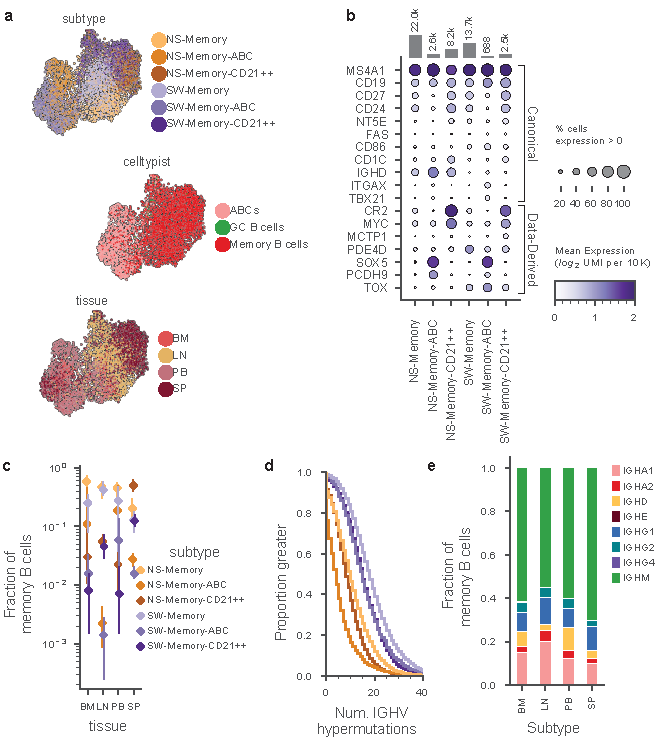
\includegraphics[width=12cm, keepaspectratio]{figs/Tabula_Bursa/EDFigure2_MemB_subtypes.pdf}
    \caption[Heterogeneity in memory B cells.] {(a) Low-dimensional (UMAP) representation of transcriptional heterogeneity in memory B cells. Celltypist labels (top), (middle) transcriptome-derived labels, and tissue (bottom). For these UMAPs, celltypes were sampled uniformly before calculating a neighbors graph. (b) Genes distinguishing between the subtypes of memory B cells, where the top half of the plot shows canonical genes often used for flow cytometry and the bottom shows the data-derived, transcriptionally detected genes which distinguish the subtypes. (c) The relative fractional abundance of memory B subtypes in tissues averaged across all donors. (d) The distribution of  hypermutation levels. (e) Barplot of constant region usage in tissues}
    \label{ED:memoryb-overview}
\end{figure}


\begin{figure}
    \centering
    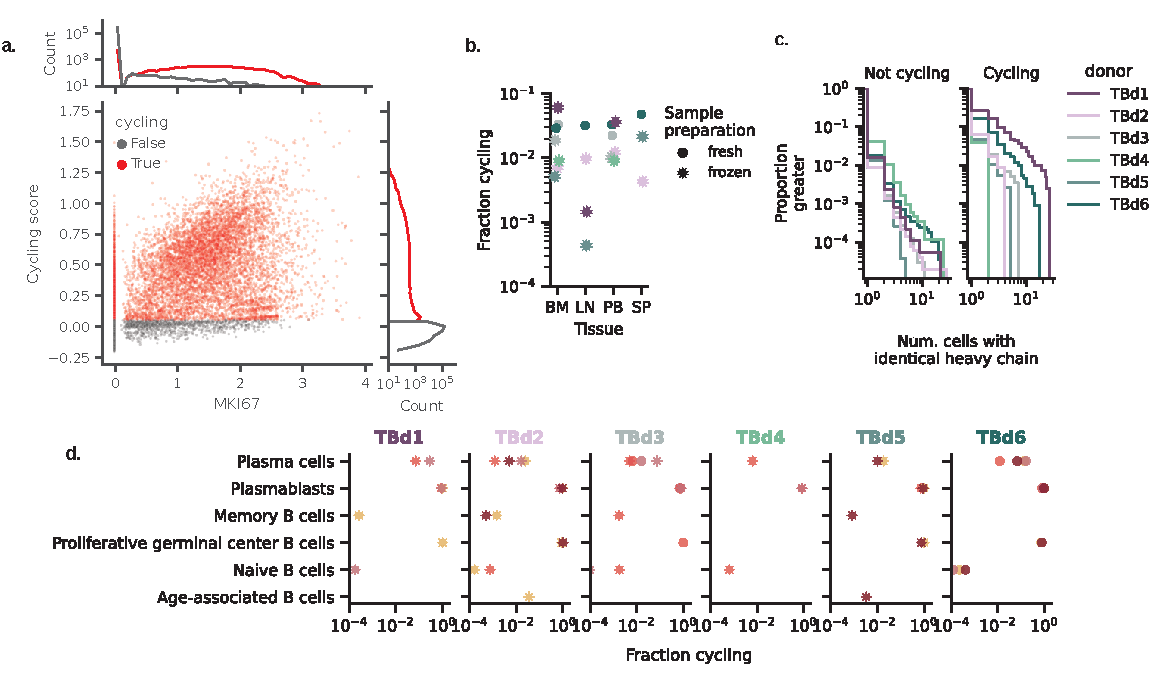
\includegraphics[width=\textwidth, keepaspectratio]{figs/Tabula_Bursa/EDFigure1.pdf}
    \caption[Cell cycle analysis across tissues.] {(a) Jointplot of the cycling score (calculated using the set of 30 genes most correlated with MKI67 expression) and normalized $log_2$ transcript counts of MKI67. (b) Fraction of cells cycling for each donor in each tissue. (c)The distribution of numbers of cells with identical VDJ sequences. (d) Fraction cycling shown for different celltypist defined cell types, with markers denoting fresh or frozen as in (b) }
\label{ED:cycling}
\end{figure}

\chapter{Concluding Remarks}
In this thesis work, I used a number of new technologies to better understand the dynamics of cellular behavoirs in the immune system. In the first work, I helped create one of the most comprehensive references to date of the molecular characteristics of human cells. In the second work, I used these new tools to comprehensively investigate B cell the molecular characteristics of their activation and differentiation. This work combined an old approach, lineage tracing, with the new single-cell transcriptomic approaches to systematically understand how clones behave in response to external stimuli. Paradoxically, I view this work as a simple proof-of-concept. The technologies I used do not yet allow the scale necessary to explore multiple axes of B cell differentiation, such as how B cells from other tissue besides the peripheral blood would respond to the same stimulus, or what the differentiation process looks like in response to a large panel of stimuli. Nonetheless, we quantitatively characterized the extent to which B cell clones propagate information about their initial states while they remodel their phentoypes in response to stimuli. In my opinion, the most important result is that even with strong over-clustering of the neighborhood graphs of transcriptomes, we see clones occupy more similar regions of the space than expected by random chance. This suggests that cell types or states are more granular in a meaningful way, than researchers had previously thought. The approaches developed there should only become more useful as the scale of these measurements increase. In the third work, we I developed a dataset which shows the B cell repertoire at unprecedented resolution. However, I like to jokingly call it an 8-bit representation of the antibody repertoire. Once again, due to scaling constraints, this is a grainy picture of the immune system. From this picture, we were able to infer key statistical properties of the human immune system, such as how much sharing of clones occurs between tissues. In addition, broadly speaking, we were able to show how B cell fate decisions are made \textit{in vivo}, and identify ever more granular sub-types of B cells.
Single cell approaches have long been a dream of biologists, as cells are the fundamental unit of biology. Indeed, the molecular biology revolution of the 1950s and 1960s was kicked-off by clever experiments which counted the progeny of single bacterial cell or phages with mutations. Now with powerful single-cell tools, I have helped create detailed pictures of the molecular contents of the cells in the body. These references will prove useful for many tasks, including diagnostic development and inferences into possible targets for therapeutics. In some ways, it appears biology is going the way of physics, where data is generated by massive consortia in multi-year, multi-million dollar projects. The trend towards making biology a data-driven science is good. However, I believe the most important advances will come from people with incisive lines of questioning, working in small groups towards the answers. New single-cell tools will never substitute for framing the right questions and designing the right experiments. Incisive follow-on investigations, will be aided by these atlasing and profiling efforts, but focused work on fundamental questions of general interest is more important than ever. The next suite of biological tools are the ones are likely to create the next biological revolution if they can combine the unbiased data-generation exemplified here with facile re-programming of cells.      


% uncomment below if you have an appendix
% \appendix
% \chapter{A Long Proof}

\bibliographystyle{unsrt}  % can change to fit your field e.g. pnas2009
\bibliography{mybib}  % no .bib extension necessary

% adds a non-numbered signature page at end (for printing on ACID-FREE paper)
% (remember to comment out when submitting final version)
\onlinesignature

\end{document}
